\section{Το πρόβλημα της πρόβλεψης ακολουθιών}

	Τα σύνορα της τεχνητής νοημοσύνης εκτείνονται πέρα από το παραδοσιακό πρόβλημα της εκμάθησης ενός στατικού συνόλου δεδομένων με επιβλεπόμενες μεθόδους,
	όπως γίνεται σε πολλές σύγχρονες εφαρμογές \parencite{lecun}.
	Η τεχνητή νοημοσύνη καλείται σήμερα να αξιοποιήσει τις καταιγιστικές ροές δεδομένων που παρέχει το (ανθρωπογενές και μη) περιβάλλον, σε πραγματικό χρόνο,
	και δίχως την πολυτέλεια της προσήμανσης που απαιτεί η επιβλεπόμενη μάθηση ---
	εφαρμογές Internet of Things που απαιτούν δυναμική αλληλεπίδραση με το περιβάλλον τους έρχονται στο μυαλό \parencite{mohammadiDeepLearningIoT2018}.

	Επομένως, καλούμαστε να μοντελοποιήσουμε έναν κόσμο που αλλάζει \parencite{staticbottleneck}.
	Το μοντέλο οφείλει ή να είναι γενικότερο από όλες τις δυνατές μεταβολές του κόσμου ή να αλλάζει μαζί του.
	Η έννοια της ροής δεδομένων που αναφέρθηκε υπονοεί την έννοια του χρόνου, της αλληλουχίας, που επιτρέπει στο μοντέλο να αντλήσει πληροφορία από την αιτιώδη σχέση.
	Την ερμηνεία του κόσμου με τη βοήθεια της συνεπαγωγής και της αναγνώρισης απαιτήσεων και συνεπειών.

	Ορίζεται έτσι το πρόβλημα της εκμάθησης και πρόβλεψης ακολουθιών.
	Δηλαδή, ο πράκτορας που παρακολουθεί μια αλληλουχία δεδομένων (γεγονότων) καλείται να προβλέψει τη συνέχεια και να δράσει έτσι, ώστε βέλτιστα να ανταμειφθεί.
	Η ανταμοιβή, το κίνητρο και γενικότερα ο στόχος έχουν τεθεί από εξωτερικό παράγοντα και βρίσκονται εκτός του πλαισίου του προβλήματος.
	Άμεση εφαρμογή της πρόβλεψης είναι και η αναγνώριση ανωμαλιών.

	Η εκμάθηση ακολουθιών είναι κλασικό πρόβλημα, για το οποίο έχουν αναπτυχθεί κλασικές λύσεις.
	Κυριότερο και ευρύτερα διαδεδομένο είδος μοντέλων, ειδικά πριν τη σύγχρονη επάνοδο των νευρωνικών δικτύων, είναι τα Hidden Markov Models (\ref{fig:HMM}).
	Από το πεδίο των κλασικών νευρωνικών δικτύων προσφέρεται η λύση των νευρωνικών δικτύων χρονικής καθυστέρησης (TDNN).
	Η ουσιαστική συνεισφορά των κλασικών νευρωνικών δικτύων επιτυγχάνεται όμως με τα ανάδρομα δίκτυα (RNN),
	που γενίκευσαν τις παλαιότερες προσθιοδρομικές (feedforward) αρχιτεκτονικές ακριβώς για να μπορούν να αντιμετωπίσουν εγγενώς προβλήματα ακολουθιών.
	Ιδιαίτερης μνείας χρήζει η δομή «μακράς βραχυπρόθεσμης μνήμης» (LSTM).
	Από το 2015 έχει χρησιμοποιηθεί με επιτυχία σε ποικίλες εφαρμογές πολύ πιο σύνθετες από την εισαγωγή που παρουσιάζεται εδώ,
	όπως ως τεχνητή νοημοσύνη που παίζει το παιχνίδι StarCraft 2 \parencite[AlphaStar][]{vinyalsAlphaStarMasteringRealTime2019}.

	\begin{figure}
		\centering
		\begin{subfigure}[t]{0.52\textwidth}
			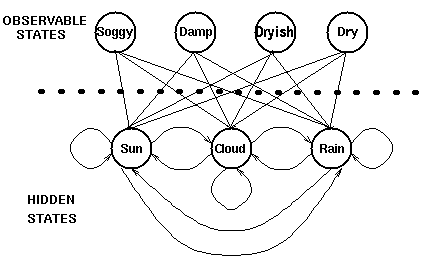
\includegraphics[width=\textwidth]{figures/hmm}
		\end{subfigure}
		\hfill
		\begin{subfigure}[t]{0.47\textwidth}
			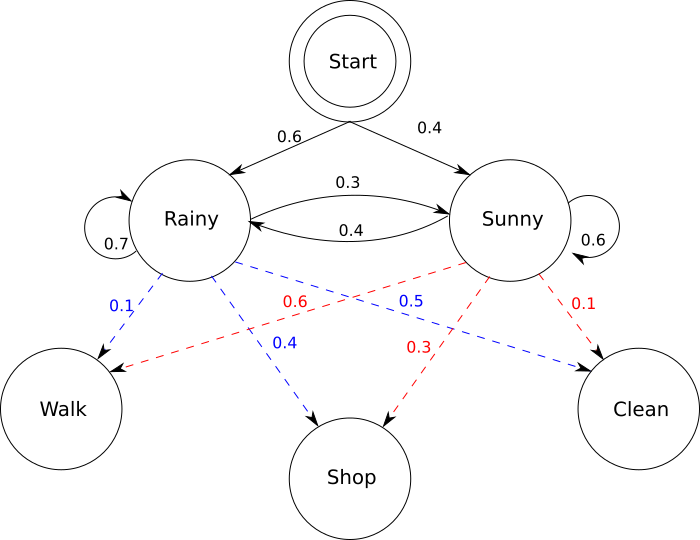
\includegraphics[width=\textwidth]{figures/hmm2}
		\end{subfigure}
		\caption[hidden markov model]{Hidden Markov Model}
		\label{fig:HMM}
	\end{figure}

	Σε αυτόν το χώρο λύσεων υπάρχουν παρόλα αυτά σημεία για βελτίωση.
	Οι περισσότερες εφαρμογές, συμπεριλαμβανομένου του AlphaStar, βασίζονται σε επιβλεπόμενη και ενισχυτική μάθηση,
	αφήνοντας ευρύ πεδίο εξερεύνησης για μη επιβλεπόμενα μοντέλα.
	Καθώς ο όγκος των ροών δεδομένων αυξάνεται εκθετικά \parencite{losingIncrementalOnlineLearning2018},
	παρατηρείται αυξανόμενη ζήτηση για αλγορίθμους που προσαρμόζονται γρήγορα στις εξελισσόμενες στατιστικές των δεδομένων τους (συνεχής μάθηση),
	έχοντας πρόσβαση μόνο σε μικρό χρονικό παράθυρο πληροφορίας.
	Στην προσπάθεια αυτή αναπτύσσονται ενεργά τεχνικές για βελτίωση της αποδοτικότητας δειγμάτων της μάθησης \parencite[όπως][]{nachumDataEfficientHierarchicalReinforcement2018},
	ή για παράκαμψη του προβλήματος, όπως η μεταφορική μάθηση (transfer learning) \parencite{xiongApplicationTransferLearning2018}.
	\medskip

	Στην ανάλυση των διαφόρων τρόπων ορισμού της τεχνητής νοημοσύνης, ο Wang \parencite{wangWhatYouMean2008} αναγνωρίζει τη μέθοδο
	«από τη δομή» για την έρευνα σε συστήματα που εμπνέονται ή μιμούνται
	το βασικό παράδειγμα ευφυούς συστήματος που επιλύει διαρκώς το παραπάνω πρόβλημα: τον εγκέφαλο, και ειδικά το φλοιό.
	Παρατηρείται μια τάση στο χώρο των τεχνητών νευρωνικών δικτύων ανασκόπησης της επαφής τους με τη βιολογική πραγματικότητα τα τελευταία χρόνια,
	όπως στο \cite{bengioBiologicallyPlausibleDeep2015}.
	Το πιο ηχηρό παράδειγμα είναι ο μηχανισμός κάψουλας που πρότειναν ο Hinton και συνεργάτες \parencite{sabourMatrixCapsulesEM2018,sabourDynamicRoutingCapsules2017}.
	\smallskip

	Σε αυτό λοιπόν το πλαίσιο, η μελέτη της HTM κρίνεται ιδιαίτερα καίρια.

\section{Στοιχεία της Hierarchical Temporal Memory}

	Παρακάτω θα αναφερθούμε πάλι σε στοιχεία νευροεπιστήμης.
	Καθώς ο σκοπός της περιγραφής είναι η κατανόηση των αλγορίθμων HTM, πρέπει να γίνει αποδεκτή μια παρέκκλιση από την αυστηρότητα, χάριν απλότητας.
	Σε ό,τι βιολογικό στοιχείο αναφερθεί, ο αναγνώστης ας έχει υπόψιν ότι η πραγματικότητα είναι πάντα πιο πολύπλοκη και ότι εδώ παρουσιάζονται \textit{χρήσιμες προσεγγίσεις}.

	Η κεντρική θέση στην οποία βασίζεται η Hierarchical Temporal Memory τμηματοποιεί τον εγκεφαλικό φλοιό σε ένα ψηφιδωτό βασικών μονάδων επεξεργασίας,
	των \textbf{«φλοιικών στηλών» (cortical columns)},
	που έχουν την ίδια δομή καθεμία και εκτελούν τους \textbf{ίδιους αλγορίθμους, αλλά σε διαφορετικά δεδομένα}.
	Η ιδέα αυτή έχει μακρά ιστορία στη νευροεπιστήμη, με μια συγκεντρωτική επισκόπηση από Defelipe, Markram κ.ά \cite{defelipeNeocorticalColumn2012}
	να την οριοθετεί και να παρουσιάζει την ευρεία χρήση και κακομεταχείριση του όρου.
	Για παράδειγμα, η εισαγωγική πρόταση περί «ψηφιδωτού» παραπάνω πρέπει να αντιμετωπιστεί μόνο ως πρώτη προσέγγιση,
	γιατί οι στήλες δε φέρονται να εχουν γεωμετρικά σαφή σύνορα μεταξύ τους, αλλά διάχυτες ζώνες μετάβασης.
	Πρεσβευτής και βασικός αποκρυσταλλωτής της ιδέας είναι ο Mountcastle \parencite{mountcastleColumnarOrganizationNeocortex1997},
	με την ιδέα να χαίρει τόσο αποδοχής \parencite{haueisLifeCorticalColumn2016}, όσο και κριτικής ως προς τη χρησιμότητά της \parencite{hortonCorticalColumnStructure2005}.
	Παρόλα αυτά, εδώ θα την υιοθετήσουμε.
	Έτσι, ο εγκεφαλικός φλοιός αποδομείται σε πλειάδα μονάδων επεξεργασίας κοινής αρχής, και οι αλγόριθμοι που θα παρουσιαστούν περιγράφουν τη λειτουργία της μονάδας.

	Η φλοιική στήλη είναι λοιπόν ένας \textbf{πληθυσμός νευρώνων με κοινή συνδεσμολογία}: \textit{λαμβάνουν το σήμα εισόδου από κοινές πηγές και στέλνουν το σήμα εξόδου σε κοινούς παραλήπτες}.
	Συχνά, τέτοιοι παραλήπτες είναι άλλες φλοιικές στήλες.
	Συντάσσονται έτσι επεξεργαστικές \textbf{ιεραρχίες}, με τα πρώτα στάδια της ιεραρχίας να δημιουργούν απλούστερα μοντέλα για τον κόσμο από τα μετέπειτα
	(κυρίως γιατί τα μετέπειτα συγκεντρώνουν περισσότερη πληροφορία).

	Οι νευρώνες στους οποίους αναφερόμαστε παραπάνω, οι πυραμιδικοί νευρώνες, βρίσκονται κάθε στιγμή σε 1 από 2 καταστάσεις: ενεργοί ή ανενεργοί.
	Η ενεργοποίησή τους («δυναμικό δράσης») ερεθίζει άλλους νευρώνες με τους οποίους συνδέονται και μπορεί να τους οδηγήσει σε ενεργοποίηση.
	Μπορούμε λοιπόν να περιγράψουμε την κατάσταση του φλοιού κάθε στιγμή ως το σύνολο των νευρώνων που είναι ενεργό.
	Προκύπτει ότι το σύνολο αυτό είναι πολύ μικρό ποσοστό του συνολικού νευρικού πληθυσμού, δηλαδή η ενεργοποίηση είναι \textbf{αραιή}, περίπου 2\%.
	Σημειώνεται ότι οι πυραμιδικοί νευρώνες είναι η μειοψηφία των νευρώνων στο φλοιό.
	Το βασικό κοινό τους χαρακτηριστικό είναι ότι στέλνουν τους άξονές τους μέσω της λευκής ύλης σε μακρινούς προορισμούς, για το οποίο και ονομάζονται κύριοι νευρώνες.
	Περισσότεροι είναι οι διάμεσοι νευρώνες (interneurons), των οποίων οι άξονες παραμένουν σε μικρή εμβέλεια, και θεωρείται ότι συμμετέχουν σε τοπικά κυκλώματα
	που εν τέλει ρυθμίζουν την ενεργοποίηση των κυρίων νευρώνων \parencite{freundInterneurons2008}.

	Το μοτίβο ενεργοποίησης ενός πληθυσμού νευρώνων της ίδιας στήλης αποτελεί στο πλαίσιο της θεωρίας HTM τη δομή δεδομένων του εγκεφάλου
	και ονομάζεται \textbf{αραιή διανεμημένη αναπαράσταση (SDR)}.
  Τα SDR αναλύονται στην ενότητα \ref{htm:sdr}.
	Κάθε αίσθηση στέλνει SDR στις στήλες που την επεξεργάζονται\char"0387  κάθε στήλη στέλνει SDR στους μύες ή σε άλλες στήλες ως έξοδο.
	Η είσοδος σε ένα μοντέλο HTM πρέπει επομένως να μεταφράζει τη φυσική ποσότητα που θέλουμε να επεξεργαστούμε σε SDR, με τη διαδικασία να ονομάζεται \textbf{κωδικοποίηση}.
	Αντίστοιχα, η ερμηνεία ενός SDR εξόδου ονομάζεται \textbf{αποκωδικοποίηση}.

	Από τους κοινούς αλγορίθμους που υλοποιεί κάθε φλοιική στήλη, η HTM αυτή τη στιγμή περιγράφει 2: τη \textbf{χωρική συγκέντρωση} και τη \textbf{χρονική μνήμη}.
	Η χρονική συγκέντρωση είναι επίσης διαδικασία που υποτίθεται, αλλά δεν έχει περιγραφεί επαρκώς και αποτελεί βασικό σημείο για περαιτέρω μελέτη.

\subsection{Μοντέλο νευρώνα} \label{htm:model_neuron}

	\subsubsection{Νευρώνες}

	Στον ανθρώπινο εγκέφαλο υπάρχουν πολλά είδη νευρώνων, που διαφέρουν στη μορφολογία, στις ηλεκτρικές και χημικές τους ιδιότητες \parencite{markramReconstructionSimulationNeocortical2015}.
	Η μόνη κατηγορία νευρώνα στην οποία βασίζεται το νευρικό μοντέλο της HTM είναι οι πυραμιδικοί νευρώνες \ref{fig:pyramidal_neuron}
	(το αποτέλεσμα της συμπεριφοράς άλλων νευρώνων συμπεριλαμβάνεται έμμεσα στη λογική των αλγορίθμων).
	Ο πυραμιδικός νευρώνας είναι ένα σύνθετο στοιχείο, με πολλούς χώρους και διανεμημένες λειτουργίες, που υλοποιούν τις λογικές πράξεις της άθροισης,
	του πολλαπλασιασμού, της χωρικής και χρονικής ολοκλήρωσης ταυτόχρονα και παράλληλα σε διαφορετικές ομάδες εισόδων.
	Η κεντρική δομή του νευρώνα, το σώμα, δέχεται ερεθίσματα από άλλους νευρώνες.
	Αρκετά τέτοια ερεθίσματα σε σύντομο χρονικό διάστημα είναι ικανά να ενεργοποιήσουν το νευρώνα.
	Οι πηγές των σημάτων που ο νευρώνας λαμβάνει στο σώμα του ονομάζονται υποδεκτικό πεδίο (receptive field) του νευρώνα.
	Από το σώμα φυτρώνουν οι εγγύς δενδρίτες. Ο ερεθισμός τους δεν είναι ικανός συνήθως να ενεργοποιήσει το νευρώνα, αρκεί όμως για να τον θέσει
	σε κατάσταση «επιφυλακής» (αποπολωμένος/προβλεπτικός), διευκολύνοντας τη μετέπειτα ενεργοποίησή του από σωματικά ερεθίσματα.
	Ομοίως και για τον ερεθισμό απομακρυσμένων ή κορυφαίων δενδριτών κατά μήκος του άξονα.

	\begin{figure}[t]
		\centering
		\begin{subfigure}[t]{0.29\textwidth}
			\centering
			\includesvg[width=\textwidth]{figures/pyramidal_cell.svg}
			\captionsetup{singlelinecheck=off}
			\caption[πυραμιδικός νευρώνας]{%
				Τυπική μορφή πυραμιδικού νευρώνα:
				\begin{enumerate}[nosep]
					\item {\color{red} σώμα}
					\item {\color{red} βασικός δενδρίτης}
					\item {\color{red} κορυφαίος δενδρίτης}
					\item {\color{blue} άξονας}
					\item {\color{blue} παράπλευρος άξονας}
				\end{enumerate}
			}
			\label{fig:pyramidal_neuron}
		\end{subfigure}
		\hfill
		\begin{subfigure}[t]{0.6\textwidth}
			\centering
			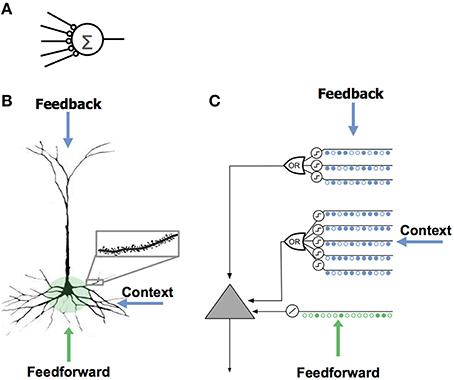
\includegraphics[width=\textwidth]{figures/numenta_neuron}
			\captionsetup{singlelinecheck=off}
			\caption[μοντέλο νευρώνα ΗΤΜ]{
				\begin{enumerate}[nosep,label=\Alph*.]
					\item Μοντέλο τυπικού νευρώνα σε τεχνητό νευρωνικό δίκτυο
					\item Αναπαράσταση πυραμιδικού νευρώνα
					\item Μοντέλο νευρώνα HTM
				\end{enumerate}
			}
			\label{fig:numenta_neuron}
		\end{subfigure}
		\caption[πυραμιδικός νευρώνας και μοντέλο νευρώνα στην HTM]{πυραμιδικός νευρώνας και μοντέλο νευρώνα στην HTM	\parencite[πηγές][]{wiki_pyramidalcell,hawkinsWhyNeuronsHave2016}}
		\label{fig:pyramidal_htm_neuron}
	\end{figure}

	Στο πλαίσιο της HTM, νευρώνα ονομάζουμε μια δομή που δέχεται ερεθίσματα στους δενδρίτες της και τροποποιεί την τρισταθή της κατάσταση με βάση αυτά.
	Η κατάσταση μπορεί να είναι \textit{ανενεργή, αποπολωμένη (αλλιώς προβλεπτική) ή ενεργή}.
	Όπως φαίνεται στο σχήμα \ref{fig:numenta_neuron}, ο νευρώνας HTM έχει 3 πύλες εισόδου.
	Ερεθίσματα στην προσθιοδρομική (feedforward) είσοδο προσμετρώνται και, αν ξεπεράσουν ένα κατώφλι, ο νευρώνας μεταβαίνει στην ενεργή κατάσταση.
	Ερεθίσματα στην είσοδο συμφραζομένων (context) είναι ικανά να προκαλέσουν αποπόλωση σε ανενεργό νευρώνα, αλλά όχι να τον ενεργοποιήσουν.
	Ομοίως και στην αναδρομική (feedback) είσοδο.
	Προσομοιώνονται έτσι μερικές συμπεριφορές του βιολογικού πυραμιδικού νευρώνα.
	Σε αντιπαραβολή, ο νευρώνας ενός κλασικού τεχνητού νευρωνικού δικτύου δεν έχει διακριτά λειτουργικά τμήματα.
  Αθροίζει μαζί όλα τα ερεθίσματα που λαμβάνει στη μία είσοδό του.

	\subsubsection{Συνάψεις}

	Η δομή που μεταφέρει σήματα μεταξύ νευρώνων ονομάζεται \textit{σύναψη} και είναι κατά κανόνα \textbf{μονόδρομη}.
	Συνάψεις σχηματίζονται στο σημείο επαφής δύο νευρώνων, του προσυναπτικού και του μετασυναπτικού, συνήθως από τον άξονα του προσυναπτικού σε δενδρίτη ή στο σώμα του μετασυναπτικού.
	Στο φλοιό οι συνάψεις είναι χημικής φύσεως, όχι ηλεκτρικής.
	Όταν το δυναμικό δράσης του προσυναπτικού νευρώνα φθάσει σε σύναψη, προκαλεί την απελευθέρωση νευροδιαβιβαστών στον εξωκυττάριο χώρο,
	προς την κατεύθυνση του μετασυναπτικού νευρώνα.
	Ο μετασυναπτικός νευρώνας φέρει υποδοχείς που ανιχνεύουν την παρουσία νευροδιαβιβαστών και συμμετέχουν στην αποπόλωση ή υπερπόλωση του νευρώνα τους.
	Αυτός ο μηχανισμός εγγυάται τη μονόδρομη μεταγωγή σήματος δια μέσου της σύναψης.
	Εν τω βάθει ανάλυση του αντικειμένου παρουσιάζεται στο \cite{kandelPrinciplesNeuralScience2013}.

	Οι συνάψεις χωρίζονται σε 2 κατηγορίες: διεγερτικές και ανασταλτικές.
	Η ενεργοποίηση μιας διεγερτικής σύναψης καθιστά πιο πιθανή την πρόκληση δυναμικού δράσης στο μετασυναπτικό νευρώνα,
	ενώ η ενεργοποίηση ανασταλτικής σύναψης την καθιστά λιγότερο πιθανή.
	Ένας τύπος προσυναπτικού νευρώνα δημιουργεί έναν τύπο συνάψεων: οι πυραμιδικοί δημιουργούν διεγερτικές και οι περισσότεροι διάμεσοι νευρώνες ανασταλτικές.
	Ο ίδιος νευρώνας όμως δέχεται σήματα και από διεγερτικές και ανασταλτικές συνάψεις, που ανταγωνίζονται μεταξύ τους.
	Οι διεγερτικές συνάψεις φέρουν συγκεκριμένους νευροδιαβιβαστές, με πιο συχνό το γλουταμικό.
	Οι ανασταλτικές χρησιμοποιούν διαφορετικούς, όπως το GABA.

	Συνάψεις υπάρχουν σε όλες τις ζώνες ερεθισμού που αναφέρθηκαν:
	στο σώμα, στους εγγύς και κορυφαίους δενδρίτες.
	Οι συνάψεις είναι επίσης ο στόχος των μηχανισμών μάθησης/προσαρμογής.
  Χαρακτηρίζονται από μία μεταβλητή, ένα μέγεθος, που προσαρμόζεται με κανόνες που εμπίπτουν στον όρο «Hebbian learning»,
	συγκεκριμένα, «πλαστικότητα εξαρτώμενη από το χρονισμό των ερεθισμάτων» (spike timing-dependent plasticity, STDP) \parencite{songCompetitiveHebbianLearning2000}.
	Στο πλαίσιο της HTM όμως το μέγεθος \textbf{δε συνεπάγεται συναπτικό βάρος}: οι συνάψεις είναι συνδεδεμένες ή αποσυνδεδεμένες.
	Μια σύναψη με πολύ μικρό μέγεθος θεωρείται αποσυνδεδεμένη και δε μετάγει καθόλου ερεθίσματα.
	Καθώς μεγαλώνει, εφόσον περάσει ένα κατώφλι γίνεται συνδεδεμένη και μετάγει ερεθίσματα.
  Το μέγεθος δηλαδή της σύναψης κρίνει πόσο εύκολα η σύναψη θα συνδεθεί ή αποσυνδεθεί, και γι'αυτό ονομάζεται μονιμότητα.

	\begin{wrapfigure}{R}{0.56\textwidth}
		\centering
		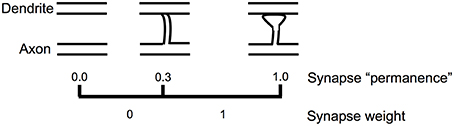
\includegraphics[width=0.55\textwidth]{figures/synapse_permanence}
		\caption[μονιμότητα σύναψης]{Μονιμότητα σύναψης}
		\label{fig:synapse_permanence}
	\end{wrapfigure}

	Ένας πυραμιδικός νευρώνας μπορεί να έχει χιλιάδες συνάψεις. Ελάχιστες από αυτές βρίσκονται κοντά στο σώμα και, όπως προαναφέρθηκε, μπορούν να τον ενεργοποιήσουν.
	Οι υπόλοιπες βρίσκονται στους δενδρίτες και, μεμονωμένα, έχουν πολύ μικρή επίδραση στο σώμα.
	Οι δενδρίτες όμως προκύπτει ότι παίζουν ρόλο σύνθετων επεξεργαστικών στοιχείων.
	Αν ενεργοποιηθούν \textit{περισσότερες από 8-20 συνάψεις} σε μικρό χρόνο στον ίδιο δενδρίτη, τότε ο δενδρίτης ενεργοποιείται και δημιουργεί ένα δυναμικό που προκαλεί την αποπόλωση όλου του νευρώνα \parencite{hawkinsWhyNeuronsHave2016}.
  Καθώς ο δενδρίτης ενεργοποιείται μόνο αν συμπέσει χρονικά και χωρικά η ενεργοποίηση πολλών συνάψεων,
	λειτουργεί ουσιαστικά ως \textbf{«ανιχνευτής συμπτώσεων»} (coincidence detector).

  Ας εξετάσουμε γιατί αρμόζει αυτός ο όρος, μελετώντας τα μοτίβα που ενεργοποιούν τους δενδρίτες στην επόμενη ενότητα.

\subsection{Αραιές Διανεμημένες Αναπαραστάσεις (SDR)} \label{htm:sdr}

	Με βάση την παρατήρηση της αραιής ενεργοποίησης των νευρώνων στον εγκέφαλο σχεδιάζουμε ένα μεγάλο, αραιό, δυαδικό διάνυσμα που αναπαριστά την κατάσταση ενεργοποίησης κάθε νευρώνα της περιοχής που μελετούμε.
	Ουσιαστικά, αυτά τα αραιά διανύσματα αποτελούν τη «δομή δεδομένων» \cite{neuronssynapses,sdrkanerva} του εγκεφάλου.

	Αναφέρθηκε στην \ref{htm:model_neuron} ότι οι δενδρίτες λειτουργούν ως ανιχνευτές συγκεκριμένων μοτίβων ενεργοποίησης.
	Πώς όμως αρκούν 8-20 συνάψεις για να διακρίνουν συγκεκριμένα μοτίβα μέσα σε μεγάλους νευρικούς πληθυσμούς; Το κλειδί είναι η αραιή ενεργοποίηση.

	Έστω ένας πληθυσμός 200K νευρώνων, όπου ενεργοί είναι το 1\%, και ένας δενδρίτης που απαιτεί 10 ερεθίσματα για να ενεργοποιηθεί.
	Αν τυγχάνει να έχει συνδεδεμένες συνάψεις σε 10 από τους 2000 ενεργούς νευρώνες, ενεργοποιείται.
	Το «μοτίβο» εν προκειμένω είναι το σύνολο των συγκεκριμένων 2000 νευρώνων που ενεργοποιήθηκαν.
	Προφανώς, αφού έχει συνάψεις μόνο με 10/2000 ενεργούς νευρώνες, ο δενδρίτης θα μπορούσε να ενεργοποιηθεί κατά λάθος και σε πολλά διαφορετικά μοτίβα,
	που τυχαίνει να μοιράζονται τους ίδιους 10 νευρώνες με το αρχικό.
	Πόση είναι η πιθανότητα ενός τέτοιου σφάλματος; $9.8\times 10^{-21}$.

	Παρακάτω θα μελετήσουμε τις ιδιότητες των SDR για να διαπιστωθεί πώς προκύπτει αυτό το αποτέλεσμα.

	\subsubsection{Ορισμοί SDR}

	Έστω N-bit SDR $s={0,1}^N$. Ο αριθμός των μονάδων στο s $w=count(s)$ ονομάζεται πληθάριθμος.
	Η χωρητικότητα SDR με μέγεθος N και πληθάριθμο w είναι το πλήθος των διαφορετικών SDR με αυτή τη μορφή, δηλαδή οι συνδυασμοί των Ν ανά w:
	$$ \text{χωρητικότητα(N,w)}= \binom N w= \frac{N!}{w!(N-w)!} $$

	Έστω 2 SDR Α,Β μήκους Ν.
	Ορίζουμε:
	\begin{table}[h!]
	\begin{tabular}{ l|l }
		Union & $A|B$ \\
		Overlap & $A\&B$ \\
		Overlap score & $\norm{A\&B}$ \\
		Overlap set(θ) & \{K όπου $\norm{A\&K}>θ$\} \\
		Ταιριάζουν(θ) & $A \;\mathit{ταιριάζει}_θ\; B \iff {A,B} \in $ ίδιο overlap set(θ)
	\end{tabular}
	\end{table}

	\subsubsection{Ταύτιση SDR και θόρυβος}

	Ας μελετήσουμε τον ορισμό ότι δύο SDR Α με πληθάριθμο w και Β \textit{ταιριάζουν}.
	Έστω B:= A + 30\% θόρυβος τυχαίας αναστροφής bit.
	Τότε το προσδοκώμενο overlap score A,B θα είναι $70\%w$. Αν $θ:= 70\%w$, τα Α,Β προσδοκάται να ταιριάζουν.

	Το παράδειγμα αυτό μπορεί να εστιαστεί για την περίπτωση της ενότητας \ref{htm:sdr}.
	Έστω Α το SDR της ενεργοποίησης των 200Κ νευρώνων με w=2000 ενεργούς, και ο δενδρίτης που έχει συνάψεις με 30 από τους ενεργούς.
	Υπό την οπτική του δενδρίτη έχουμε το SDR $\hat{A}$ με μέγεθος 200Κ και $\hat{w}=30$, γιατί οι υπόλοιποι ενεργοί νευρώνες δεν τον ερεθίζουν.
	Αν το όριο ενεργοποίησης του δενδρίτη είναι θ=20, τότε ακόμα και με 30\% θόρυβο τυχαίας αναστροφής bit στον πληθυσμό των 200K νευρώνων
	αναμένουμε ο δενδρίτης να δεχθεί $\hat{w}_n= 70\%\hat{w}= 21 > θ$ ερεθίσματα και επομένως να ενεργοποιηθεί, παρόλο το θόρυβο.

	Θεωρήσαμε ότι το δεύτερο SDR είναι αποτέλεσμα θορύβου στο πρώτο κι επομένως ήταν θεμιτό ο δενδρίτης να τα ταυτίσει.
	Πόση όμως είναι η πιθανότητα να ενεργοποιηθεί ο ίδιος δενδρίτης από ένα διαφορετικό, τυχαίο SDR με πληθάριθμο $\hat{w}$ που δεν προκύπτει από το αρχικό;
	Σε αυτήν την περίπτωση η ενεργοποίηση θα ταύτιζε ψευδώς το τυχαίο SDR με το πρώτο.
  Η πιθανότητα ψευδούς ταύτισης είναι \footnote{υπολογίστηκε με τον κώδικα του παραρτήματος \ref{app:sdr_fp}}:
	\begin{equation}
		p_{\mathit{fp}}= \frac{ \norm{\mathit{overlap\_set(θ)}} }{ \mathit{χωρητικότητα(N,w)} }
		=	\frac{ \sum_{b=θ}^{\hat{w}} \binom{\hat{w}}{b} \binom{N-\hat{w}}{\hat{w}-b} }{ \binom N w }
		= \frac{\num{8e53}}{\num{1e4862}} = \num{5e-4809}
	\end{equation}

	Εν προκειμένω, η μικροσκοπική πιθανότητα σφάλματος οφείλεται κυρίως στο γιγαντιαίο μέτρο του χώρου (N,w).
	Η πιθανότητα τυχαίας σύγκρουσης θα ήταν όμως αμελητέα και σε πολύ μικρότερο χώρο.

	Καταδεικνύεται έτσι ότι η αναγνώριση SDR είναι μια διαδικασία \textit{ανθεκτική στο θόρυβο}.
	Επίσης, αναφαίνεται μια \textit{σχεδιαστική ελευθερία} που προσδίδει η χρήση SDR στο σύστημα:
	ανταλλαγή μεγέθους με ευρωστία στο θόρυβο.

	\subsubsection{Ταχεία ανάκληση SDR και παράλληλα ενδεχόμενα}

	Έστω ότι παρατηρούμε μια ακολουθία από SDR $\{s_t\}$.
	Κάποια χρονική στιγμή $t_0$ ρωτούμε αν έχουμε δει στη μέχρι τώρα ακολουθία $\{s_{0..t_0}\}$ το SDR Q.
	Πώς μπορούμε να απαντήσουμε γρήγορα σε αυτό το ερώτημα;

	Εφόσον γινεται δεκτή μια πιθανότητα σφάλματος, που μπορεί να προσδιοριστεί ως προς τα μεγέθη και τον πληθάριθμο των SDR όπως παραπάνω,
	δε χρειάζεται να έχουμε αποθηκεύσει όλη την ακολουθία $\{s_{0..t_0}\}$ και να συγκρίνουμε κάθε στοιχείο με το Q.
	Αντίθετα, διατηρούμε μόνο την ένωση U των SDR που έχουν προηγηθεί και συγκρίνουμε το Q με το U.

	Κάθε χρονική στιγμή,
	$$ U_t = U_{t-1} | s_t $$
	όπου $|$: δυαδικό OR

	Προφανώς,
	\begin{align*}
	 B \;\mathit{ταιριάζει}_θ\; s_i &\implies B \;\mathit{ταιριάζει}_θ\; U \\
	 B \;\mathit{ταιριάζει}_θ\; U   &\centernot{\implies} \exists i: B \;\mathit{ταιριάζει}_θ\; s_i
	\end{align*}
	γιατί ενδέχεται τμήματα του B να ταιριάζουν με τμήματα από διαφορετικά $s_i$.
	Ακολουθώντας όμως τη λογική της προηγούμενης παραγράφου, για επαρκώς αραιά $s_i, U$ η πιθανότητα σύγκρουσης είναι αρκετά μικρή.
	Οπότε μπορούμε να δεχθούμε το συμπέρασμα
	$$ B \;\mathit{ταιριάζει}_θ\; U \simplies[p] \exists i: B \;\mathit{ταιριάζει}_θ\; s_i $$
	με μια πιθανότητα σφάλματος $p$.

	Αν τα ${s_t}$ είναι μεταξύ τους ανεξάρτητα και η αραιότητά τους προκύπτει από δειγματοληψία Bernoulli με πιθανότητα ανά θέση $p$,
	τότε το $U_t$ επίσης προκύπτει από δειγματοληψία Bernoulli, με πιθανότητα ανά θέση $1-(1-p)^t$.
	Ακόμα και για αρκετά αραιά $s_t$, καθώς το $t$ αυξάνει το $U$ γρήγορα γίνεται πυκνό.
	Καθώς γίνεται πυκνό, η πιθανότητα σφάλματος $p$ αυξάνεται και το συμπέρασμα χάνει την αξία του.
	Επομένως, αυτή η μέθοδος είναι χρήσιμη μόνο όταν ο αριθμός των ανεξάρτητων $s_t$ που συγχέουμε στο U είναι ελεγχόμενος.

	Αν όμως ερμηνεύσουμε τα $s_t$ ως πεπερασμένου αριθμού διακριτά ενδεχόμενα και το U είναι η δραστηριότητα ενός πληθυσμού νευρώνων,
	ο μηχανισμός αυτός επιτρέπει στον πληθυσμό να κωδικοποιεί τα διακριτά ενδεχόμενα παράλληλα
	και να μπορέσει, όταν έχει περισσότερη πληροφορία υπό τη μορφή συνθήκης S,
	να επιλύσει την αμφιβολία περιορίζοντας τη δραστηριότητά του στο $U\&S$


\subsection{Μοντέλο δικτύου}

	\begin{figure}
		\centering
		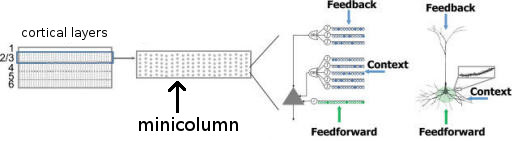
\includegraphics[width=0.9\textwidth]{figures/layer-minicolumn}
		\caption[αποδόμηση φλοιικού επιπέδου και μικροστήλες]{\textit{Αποδόμηση φλοιικού επιπέδου και μικροστήλες}.
		Μία φλοιική στήλη του νεοφλοιού αποτελείται από 6 επίπεδα νευρώνων και φαίνεται αριστερά.
		Αν πάρουμε ένα από τα επίπεδα, θα έχει πάχος μερικών νευρώνων.
		Οι νευρώνες του ίδιου επιπέδου που είναι τοποθετημένοι κατακόρυφα ορίζουν (σε πρώτη προσέγγιση) μια μικροστήλη.
		\parencite[πηγή][(τροποποιημένο)]{cuiContinuousOnlineSequence2016}
		}
		\label{fig:layer-minicolumn}
	\end{figure}

	Ο νεοφλοιός, όπως αναφέρθηκε στην ενότητα \ref{intro:brain_anatomy}, δομείται συνήθως από 6 επίπεδα νευρώνων.
	Μία φλοιική στήλη χωρισμένη στα 6 επίπεδα φαίνεται στο σχήμα \ref{fig:layer-minicolumn}.
	Ορίσαμε τη φλοιική στήλη με βάση την κοινή συνδεσμολογία των νευρώνων της, καθώς τα ερεθίσματα έρχονται από και φεύγουν προς κοινές περιοχές.
	Έτσι παρουσιάσαμε τους νευρώνες της στήλης ως πληθυσμούς που κωδικοποιούν μία κοινή οντότητα --- το βασικό τμήμα των εγκεφαλικών κυκλωμάτων.
	Είναι ακριβέστερο να μεταφέρουμε τον ορισμό αυτό από τη στήλη σε κάθε επίπεδο της στήλης.
	Μέσα σε μία στήλη δηλαδή τα 6 επίπεδα σχηματίζουν ξεχωριστά κυκλώματα, που όμως σχετίζονται μεταξύ τους και παίζουν διαφορετικούς λειτουργικούς ρόλους.
	Μία υπόθεση για τη συνδεσμολογία των επιπέδων στο τωρινό πλαίσιο της θεωρίας HTM φαίνεται στο σχήμα \ref{fig:layers-in-column}.
  Οι αλγόριθμοι που μελετούμε σε αυτήν την εργασία περιγράφουν κυρίως το επίπεδο 4 του σχήματος \ref{fig:layers-in-column}, που λαμβάνει είσοδο από τις αισθήσεις.
	Επίσης, εφεξής όταν γίνεται αναφορά σε \textit{«επίπεδο»} θα εννοείται η τομή ενός επιπέδου και μιας στήλης, δηλαδή ένα στοιχειώδες κύκλωμα.

	\subsubsection{Μικροστήλες}

	Το ελάχιστο νευρικό κύκλωμα, τόσο στο νεοφλοιό, όσο και στην HTM, είναι η μικροστήλη (minicolumn).
	Σε μία μικροστήλη ανήκουν νευρώνες που λαμβάνουν ερεθίσματα στις εγγύς συνάψεις τους από τις ίδιες συνδέσεις μακρινής απόστασης
	(από τους ίδιους νευρώνες των περιοχών που στέλνουν είσοδο).
	Δηλαδή, οι νευρώνες μιας μικροστήλης μπορούμε να θεωρήσουμε ότι έχουν \textit{ίδια είσοδο στις εγγύς συνάψεις τους
	και διαφέρουν μόνο ως προς την είσοδο στις απομακρυσμένες και κορυφαίες συνάψεις}.
	Για περισσότερες πληροφορίες στην οργάνωση των νευρώνων σε στήλες και μικροστήλες προτείνεται η θεμελιώδης εργασία των Markram et al
	«Reconstruction and simulation of neocortical microcircuitry» \parencite{markramReconstructionSimulationNeocortical2015}.

	{
	\begin{wrapfigure}{R}{0.40\textwidth}
		\centering
		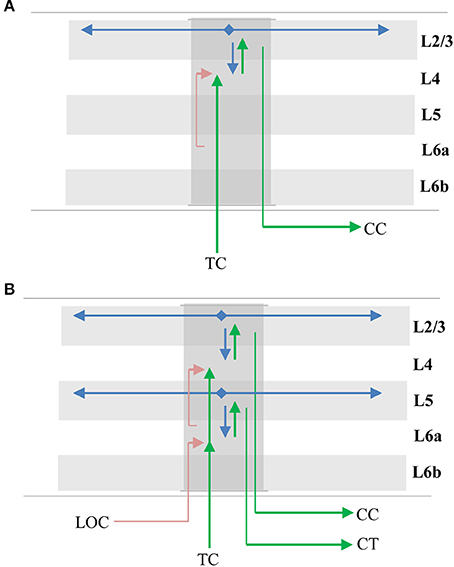
\includegraphics[width=0.39\textwidth]{figures/layers_in_column}
		\captionsetup{singlelinecheck=off}
		\caption[επίπεδα σε φλοιική στήλη]{Επίπεδα μέσα σε μία στήλη νεοφλοιού.
			Το μοντέλο συνδεσμολογίας που επισημαίνεται είναι τρέχουσα υπόθεση της θεωρίας HTM.
			\begin{itemize}[leftmargin=*]
				\item {\color{green}Προσθιοδρομική ροή ερεθισμάτων} (εγγύς συνάψεις)
				\item {\color{blue}συμφραζόμενα} (απομακρυσμένες/κορυφαίες συνάψεις)
				\item {\color{red}σήμα θέσης} (απομακρυσμένες συνάψεις, εκτός πεδίου μελέτης αυτής της εργασίας)
			\end{itemize} \parencite[πηγή][]{hawkinsTheoryHowColumns2017}
		}
		\label{fig:layers-in-column}
	\end{wrapfigure}

	Καθώς οι εγγύς συνάψεις μεταφέρουν τη βασική πληροφορία που αναπαριστά ο πληθυσμός των νευρώνων ενός επιπέδου
	κι οι απομακρυσμένες τον ρυθμίζουν με βάση συμφραζόμενα,
	οι μικροστήλες επιτρέπουν σε μια μικρή ομάδα 10-20 νευρώνων να κωδικοποιεί \textit{τα ίδια σύμβολα σε διαφορετικά συμφραζόμενα}.
	Όλοι οι νευρώνες της μικροστήλης μοιράζονται το ίδιο υποδεκτικό πεδίο, ενώ μεταξύ τους υπάρχει ανταγωνισμός.

	Όπως αναφέρθηκε στην ενότητα \ref{htm:model_neuron}, υπάρχουν τόσο διεγερτικές, όσο και ανασταλτικές συνάψεις, και κατ'επέκταση διεγερτικοί και ανασταλτικοί νευρώνες.
	Οι νευρώνες μίας μικρoστήλης έχουν βρόχο ανάδρασης μέσω ενός ανασταλτικού διάμεσου νευρώνα.
	Αν κάποιος νευρώνας της μικροστήλης ενεργοποιηθεί λίγο νωρίτερα από τους υπόλοιπους, είναι ικανός να προκαλέσει την ενεργοποίηση του διάμεσου που τους εμπλέκει,
	ο οποίος με τη σειρά του να αποτρέψει την ενεργοποίηση όσων νευρώνων δεν έχουν προλάβει να ενεργοποιηθούν (σχήμα \ref{fig:minicolumn_circ}).
	Η ενεργοποίηση του νευρώνα είναι μια εύρωστη διαδικασία που υπόκειται σε θετική ανάδραση.
	Οπότε, αναστολή μετά την ενεργοποίηση δε θα επιφέρει ουσιαστικό αποτέλεσμα.

  Έτσι υλοποιείται μια ανταγωνιστική αρχιτεκτονική («winner-takes-all»), όπου,
	αν κάποιοι νευρώνες είναι ήδη σε αποπολωμένη/προβλεπτική κατάσταση όταν έρθει προσθιοδρομική είσοδος που ερεθίζει το minicolumn,
	θα ενεργοποιηθούν πρώτοι και θα αποτρέψουν την ενεργοποίηση των υπολοίπων.

	\subsubsection{Μεταξύ μικροστηλών} \label{htm:sp_inhibition}

	Φαινόμενα ανταγωνισμού μέσω αμοιβαίας αναστολής προκύπτουν και μεταξύ γειτονικών μικροστηλών, με τη βοήθεια άλλων διάμεσων νευρώνων (σχήμα \ref{fig:SP_circ}).
	Το αποτέλεσμα είναι να εξασφαλίζεται ότι σε κάθε γειτονιά μόνο ένα αραιό υποσύνολο των πιο έντονα ερεθισμένων μικροστηλών θα επικρατήσει
	και θα ενεργοποιηθεί, σιγώντας τις υπόλοιπες.
	Ονομάζουμε το μηχανισμό αυτό «τοπική αναστολή».
	Στους αλγορίθμους που ακολουθούν, αντίθετα με τον εγκέφαλο, δεν είναι απαραίτητο να θεωρήσουμε ότι σχηματίζονται τοπικά γειτονιές\char"0387
	αντίθετα, μπορούμε να θεωρήσουμε ολόκληρο το επίπεδο μία γειτονιά, μηχανισμό που αποκαλείται «ολική αναστολή».
	}

	\begin{figure}[t]
		\centering
		\hfill
		\begin{subfigure}[t]{0.4\textwidth}
			\centering
			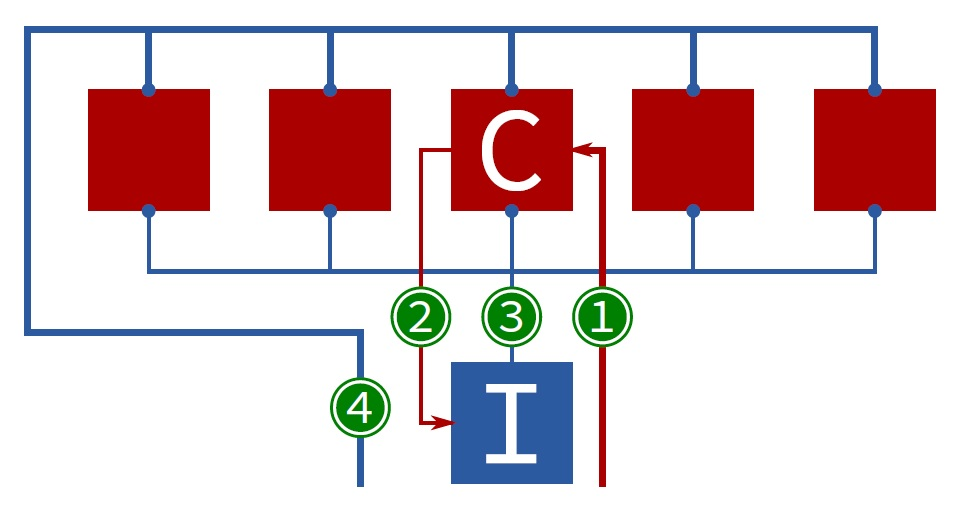
\includegraphics[width=\textwidth]{figures/spatial_hardware}
			%\captionsetup{singlelinecheck=off}
			\caption[κυκλωματική υλοποίηση χωρικού συγκεντρωτή]{Υλοποίηση χρονικού συγκεντρωτή με βάση το χρονισμό.
			Κάθε κύτταρο C αντιπροσωπεύει μία μικροστήλη. Δέχεται προσθιοδρομικά ερεθίσματα από τη ροή \circled{1}.
			Ο χρόνος που απαιτείται για την ενεργοποίηση της μικροστήλης εξαρτάται από το πόσα ερεθίσματα λαμβάνει\char"0387 μια μικροστήλη με πολλά ερεθίσματα ενεργοποιείται ταχύτερα.
			Ερεθιζόμενος με τη ροή \circled{2}, ο ανασταλτικός νευρώνας I ενεργοποιείται μετά την ενεργοποίηση προκαθορισμένου αριθμού μικροστηλών.
			Με τη ροή \circled{3} ο I αποτρέπει την ενεργοποίηση περισσότερων μικροστηλών.
			}
			\label{fig:SP_circ}
		\end{subfigure}
		\hfill
		\begin{subfigure}[t]{0.35\textwidth}
			\centering
			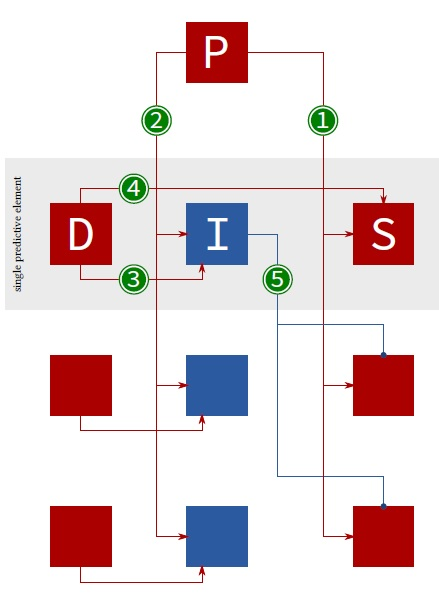
\includegraphics[width=\textwidth]{figures/temporal_hardware}
			%\captionsetup{singlelinecheck=off}
			\caption[κυκλωματική υλοποίηση μικροστήλης]{Υλοποίηση μιας μικροστήλης.
			Τα 3 στοιχεία D,I,S (δενδρίτης, αναστολέας, σώμα) μαζί περιγράφουν 1 νευρώνα.
			Το στοιχείο P είναι μοναδικό ανά μικροστήλη και είναι το ίδιο με το στοιχείο C του σχήματος (α').
			Με τη ροή \circled{1} προκαλεί την ενεργοποίηση όλων των σωμάτων της μικροστήλης.
			Όμως ο δενδρίτης (εδώ μόνο 1/κύτταρο) συγκεντρώνει ερεθίσματα από την προηγούμενη χρονική στιγμή και, αν ενεργοποιηθεί,
			προκαλεί αποπόλωση του δικού του S και I με τις ροές \circled{3},\circled{4}.
			Σε αυτήν την περίπτωση, αν στην επόμενη χρονική στιγμή το P ενεργοποιηθεί, θα ενεργοποιήσει το I,
			το οποίο με τη ροή \circled{5} θα αναστείλει τα υπόλοιπα σώματα της μικροστήλης.
			}
			\label{fig:minicolumn_circ}
		\end{subfigure}
		\hfill
		\caption[κυκλωματικές υλοποιήσεις μικροστηλών στο HICANN]{Κυκλωματικές υλοποιήσεις μικροστηλών στο HICANN \parencite{meierMixedsignalUniversalNeuromorphic2015}.
		Προσφέρουν εποπτεία της οργάνωσης των μικροκυκλωμάτων μέσω του μηχανισμού της \textit{αναστολής}.
		Σε σχέση με τη θεωρία HTM εφαρμόζουν κάποιες απλοποιήσεις, όπως μόνο 1 δενδρίτη ανά κύτταρο.
		\parencite[πηγή][]{billaudellePortingHTMModels2015}}
	\end{figure}


\subsection{Κωδικοποιητές \& αποκωδικοποιητές}

	Ο εγκέφαλος έχει ως βασικές διεπαφές με τον έξω κόσμο τον αμφιβληστροειδή χιτώνα του ματιού και τον κοχλία του αυτιού.
	Και τα 2 αυτά συστήματα μπορούμε να θεωρήσουμε ότι μετατρέπουν τα φυσικά ερεθίσματα του κόσμου σε μια πρώτη μορφή SDR,
	για να ερεθίσουν με τη σειρά τους το επόμενο επίπεδο νευρώνων.
	Το ρόλο αυτό στα συστήματα HTM παίζουν οι κωδικοποιητές.

	Οι κωδικοποιητές μπορεί να είναι από πολύ απλά έως εξαιρετικά πολύπλοκα συστήματα (βλέπε αμφιβληστροειδή).
	Ενας απλός κωδικοποιητής μπορεί να μετατρέπει ακέραιους αριθμούς συγκεκριμένου εύρους σε SDR.
	Ένας πιο σύνθετος μπορεί να παράγει SDRs από τη γεωγραφική θέση ενός αισθητήρα GPS \parencite{purdyEncodingDataHTM2016}.
	Μπορεί ακόμα να σχεδιαστεί κωδικοποιητής για λέξεις ή κείμενα, όπως κάνει η εταιρία cortical.io \parencite{semantic}.

	Ένας επιτυχημένος κωδικοποιητής πρέπει να ακολουθεί ορισμένες βασικές αρχές \parencite{purdyEncodingDataHTM2016}:
	\begin{enumerate}
		\item Είσοδοι με σημασιολογική ομοιότητα πρέπει να παράγουν SDRs με μεγάλη επικάλυψη
		\item Η ίδια είσοδος πρέπει να παράγει πάντα το ίδιο SDR
		\item Για κάθε είσοδο τα SDRs πρέπει να έχουν ίδιο μέγεθος
		\item Για κάθε είσοδο τα SDRs πρέπει να έχουν κοντινό πληθάριθμο, αρκετά υψηλό για να προσδίδει ανθεκτικότητα στο θόρυβο
	\end{enumerate}

	Αντίστοιχα με τους κωδικοποιητές, πρακτικές εφαρμογές απαιτούν και αποκωδικοποιητές.
	Ένας πρακτικός αποκωδικοποιητής θα παρουσιαστεί στην περιγραφή του πακέτου \texttt{HierarchicalTemporalMemory.jl}.
	Βασίζεται στην παρατήρηση ότι η δραστηριότητα της χρονικής μνήμης είναι η απεικόνιση ενός συμβόλου-εισόδου στο πλαίσιο των χρονικών του συμφραζομένων.
	Ο αποκωδικοποιητής που χρησιμοποιείται εδώ είναι ένα απλό ενός επιπέδου τεχνητό νευρωνικό δίκτυο που μαθαίνει να συσχετίζει
	τη δραστηριότητα της χρονικής μνήμης με τις εισόδους του κωδικοποιητή.


\section{Αλγόριθμοι της Hierarchical Temporal Memory}

Αυτή τη στιγμή στη θεωρία HTM περιγράφονται 2 βασικοί αλγόριθμοι.
Ο πρώτος κανονικοποιεί τα SDR εισόδου και ονομάζεται \textit{Χωρικός Συγκεντρωτής} (Spatial Pooler).
Ο δεύτερος μαθαίνει ακολουθίες εισόδων, εμπλουτίζοντας την αναπαράσταση της εισόδου με τα χρονικά της συμφραζόμενα, και ονομάζεται \textit{χρονική μνήμη} (Temporal Memory).

\subsection{Χωρικός Συγκεντρωτής} \label{htm:sp}

	\begin{figure}
		\centering
		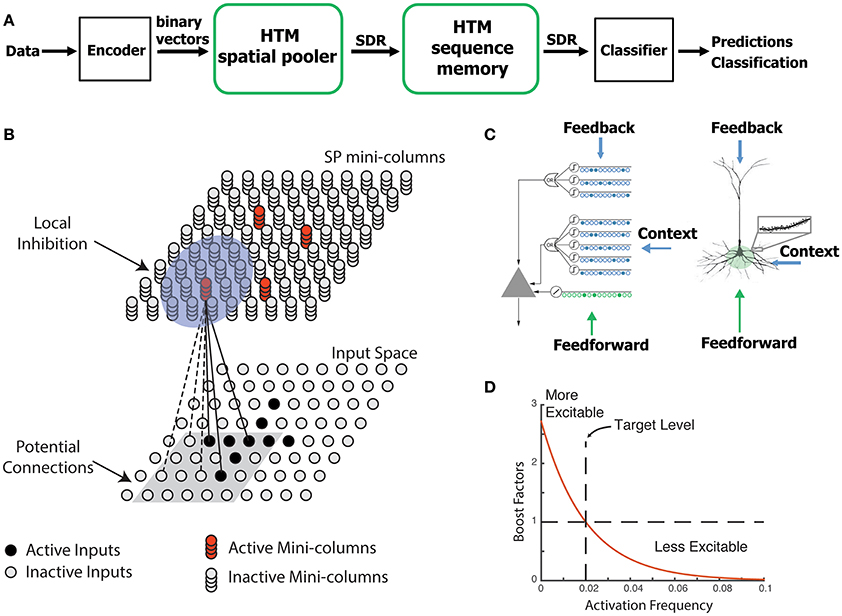
\includegraphics[width=\textwidth]{figures/numenta_spatial_pooler}
		\captionsetup{singlelinecheck=off}
		\caption[χωρικός συγκεντρωτής]{Χωρικός Συγκεντρωτής HTM.
			\begin{enumerate}[nosep,label=\Alph*.]
				\item Πλήρες σύστημα HTM για πρόβλεψη χρονοσειρών
				\item Εποπτική αναπαράσταση λειτουργίας του χωρικού συγκεντρωτή, υποθέτοντας τοπολογία (γενικά προαιρετική). Λόγω τοπολογίας, κάθε μικροστήλη έχει υποδεκτικό πεδίο ένα υποσύνολο (ολισθαίνον παράθυρο) του χώρου εισόδου, όπως φαίνεται από τη γκρίζα περιοχή. Η μπλε έλλειψη δείχνει τη γειτονιά των μικροστηλών στην οποία εφαρμόζεται τοπικός ανταγωνισμός μέσω αναστολής. Οι πλήρεις γραμμές δείχνουν συνάψεις που ισχυροποιούνται, ενώ οι διακεκομμένες, που εξασθενούν.
				\item Οι συνάψεις που συμμετέχουν στο χωρικό συγκεντρωτή είναι οι εγγύς (προσθιοδρομικές)
				\item Παρώθηση: ενίσχυση της ευαισθησίας μικροστηλών με ιστορικά σπάνια ενεργοποίηση
			\end{enumerate}
			\parencite[πηγή][]{cuiHTMSpatialPooler2017}}
		\label{fig:sp}
	\end{figure}

	Ο χωρικός συγκεντρωτής δουλεύει στο επίπεδο των μικροστηλών ενός επιπέδου, αξιοποιώντας τις εγγύς τους συνάψεις (προσθιοδρομική ροή)
	με το προηγούμενο ιεραρχικά επίπεδο (ή κωδικοποιητή) και το μηχανισμό αναστολής μεταξύ μικροστηλών που περιγράφηκε στην ενότητα \ref{htm:sp_inhibition}.
	Ο αλγόριθμος αυτός περιγράφει πώς το SDR της εισόδου ενεργοποιεί τις μικροστήλες ενός επιπέδου μέσω του ερεθισμού των εγγύς συνάψεων
	και πώς αυτές προσαρμόζονται (μαθαίνουν) με εφαρμογή ενός κανόνα «πλαστικότητας εξαρτώμενης από το χρονισμό των ερεθισμάτων» (spike timing-dependent plasticity, STDP)
	\parencite{songCompetitiveHebbianLearning2000}.
	Ο χωρικός συγκεντρωτής περιγράφεται αναλυτικά από τη Numenta στο \cite{cuiHTMSpatialPooler2017}.

	Ο στόχος του αλγορίθμου είναι \textit{να προετοιμάσει τα SDRs εισόδου για περαιτέρω επεξεργασία, εξασφαλίζοντας ορισμένες ιδιότητες}.
	Βασική αρχή λειτουργίας του είναι ότι είσοδοι που μοιάζουν μεταξύ τους (έχουν μεγάλη επικάλυψη) δημιουργούν εξόδους που μοιάζουν ανάλογα μεταξύ τους.
	Αυτή η αρχή ονοματίζει και τον αλγόριθμο.

	Οι ιδιότητες που εξασφαλίζει ο χωρικός συγκεντρωτής στα SDR εξόδου είναι:
	\begin{enumerate}
		\item \textbf{Κανονικοποίηση της αραιότητας}.
		\item \textbf{Ευρωστία στο θόρυβο}. Η έξοδος δε θα πρέπει να είναι ευαίσθητη στην παρουσία θορύβου στην είσοδο
		\item \textbf{Ανεκτικότητα στα σφάλματα}. Αν καταστραφεί ή δε λειτουργεί σωστά μέρος των νευρώνων είτε της εισόδου είτε της εξόδου, η επίδραση στο συνολικό μηχανισμό πρέπει να είναι μικρή.
		\item \textbf{Διαρκής προσαρμογή} στα εξελισσόμενα στατιστικά χαρακτηριστικά της εισόδου.
		\item \textbf{Διασπορά της ενεργοποίησης} σε όλες τις μικροστήλες του συστήματος, εξασφάλιση υψηλής εντροπίας στην ενεργοποίηση.
		\item Διατήρηση της τοπολογίας του χώρου εισόδου, εφόσον υπάρχει.
	\end{enumerate}
	Βέβαια, η ιδιότητα 5 είναι μάλλον προϋπόθεση για τις 2,3.

	Αν και αναφέρθηκε ο «αλγόριθμος» του χωρικού συγκεντρωτή, θα ήταν ακριβέστερο να δούμε το χωρικό συγκεντρωτή ως ένα δυναμικό σύστημα διακριτού χρόνου,
	με εσωτερική κατάσταση, συνάρτηση αρχικοποίησης και βήματος/μετάβασης.
	Η βασική μεταβλητή κατάστασης του χωρικού συγκεντρωτή είναι οι εγγύς συνάψεις μεταξύ της προσυναπτικής εισόδου και των μετασυναπτικών μικροστηλών του.
	Ο «αλγόριθμος» αναφέρεται ακριβέστερα σε αυτόν που υλοποιεί η συνάρτηση βήματος.

	Με την άφιξη των ερεθισμάτων από την είσοδο υπολογίζεται αρχικά η «επικάλυψη» (overlap) της εισόδου από κάθε μικροστήλη,
	δηλαδή το πλήθος ερεθισμάτων που μετήχθησαν μέσω συνδεδεμένων συνάψεων και ερέθισαν τη μικροστήλη.
	Με βάση την επικάλυψη οι μικροστήλες συμμετέχουν στον τοπικό ή ολικό ανταγωνισμό μέσω της αναστολής μεταξύ μικροστηλών,
	ώστε να προκύψουν οι αραιές μικροστήλες που θα ενεργοποιηθούν αυτή τη χρονική στιγμή.
	Μετά, προσαρμόζονται οι συνάψεις κατά STDP:
	\begin{itemize}
		\item αν η μετασυναπτική μικροστήλη ενεργοποιήθηκε, οι συνάψεις που \textit{μετήγαγαν} ερεθίσματα ισχυροποιούνται
		\item αν η μετασυναπτική μικροστήλη ενεργοποιήθηκε, οι συνάψεις που \textit{δε μετήγαγαν} ερεθίσματα εξασθενούν
		\item αν η μετασυναπτική μικροστήλη δεν ενεργοποιήθηκε, οι συνάψεις της δεν προσαρμόζονται
	\end{itemize}

	Η καλή λειτουργία του χωρικού συγκεντρωτή (ειδικά η ιδιότητα 5) υποστηρίζεται από ένα σημαντικό επικουρικό μηχανισμό ομοιόστασης που ονομάζεται \textbf{«παρώθηση»} (boosting).
	Η παρώθηση πολλαπλασιάζει την επικάλυψη κάθε μικροστήλης με έναν παράγοντα ενίσχυσης ή εξασθένισης, ανάλογα με το πόσο συχνά ενεργοποιούνταν στο πρόσφατο παρελθόν:
	ενισχύει τις μικροστήλες που ενεργοποιούνται σπάνια και εξασθενεί τις μικροστήλες που ενεργοποιούνται συχνά.
	Με αυτόν τον τρόπο επιτυγχάνει πιο ισορροπημένη συμμετοχή όλων των μικροστηλών στη χωρική κωδικοποίηση.

\subsection{Χρονική Μνήμη} \label{htm:tm}

	\begin{figure}
		\centering
		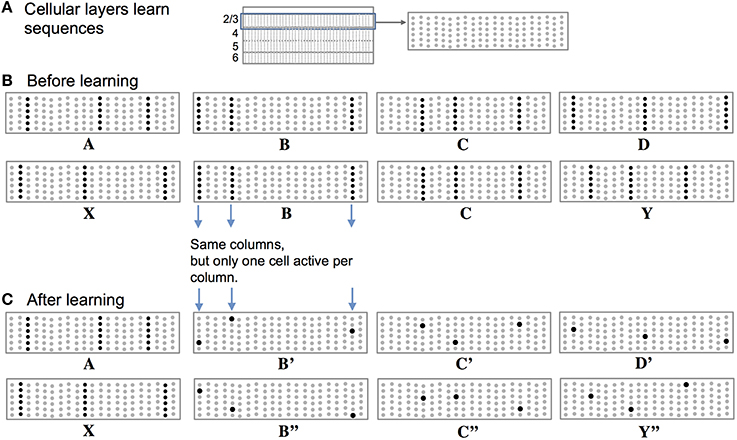
\includegraphics[width=\textwidth]{figures/numenta_temporal_memory1}
		\captionsetup{singlelinecheck=off}
		\caption[μνήμη ακολουθιών]{Αναπαράσταση ακολουθιών σε φλοιική στήλη ∩ επίπεδο.
			\begin{enumerate}[nosep,label=\Alph*.]
				\item Φλοιικά επίπεδα
				\item Ενεργοποίηση μικροστηλών σε πρωτοεμφανιζόμενη ακολουθία. Επειδή κανένα στοιχείο της ακολουθίας δεν προσδοκάται, οι μικροστήλες οδηγούνται σε έξαρση ενεργοποίησης.
				Κάθε φορά που μια μικροστήλη ενεργοποιείται απρόσμενα, δηλαδή κανένας νευρώνας της δεν προσδοκούσε την ενεργοποίησή του, ενεργοποιούνται όλοι.
				\item Έχοντας δει την ίδια ακολουθία πολλές φορές, το επίπεδο τη μαθαίνει. Συγκεκριμένα, μαθαίνει να προβλέπει την επόμενη ενεργοποίησή του, ώστε να αποφύγει την έξαρση μικροστηλών.
				Οι ίδιες μικροστήλες ενεργοποιούνται για το ίδιο σύμβολο.
				Όμως ο νευρώνας εντός της στήλης που συμμετέχει στην αναπαράσταση είναι διαφορετικός, ανάλογα με τα σύμβολα που προηγήθηκαν.
				Έτσι, κάθε σύμβολο αναπαρίσταται μαζί με τα \textit{χρονικά συμφραζόμενά} του.
			\end{enumerate}
			\parencite[πηγή][]{hawkinsWhyNeuronsHave2016}}
		\label{fig:tm}
	\end{figure}
	\begin{figure}
		\centering
		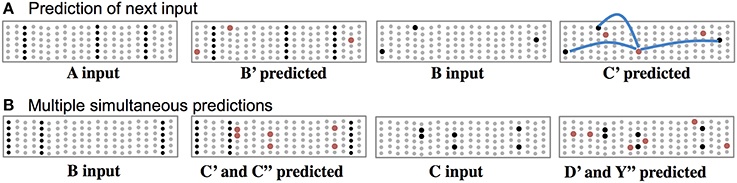
\includegraphics[width=\textwidth]{figures/numenta_temporal_memory2}
		\captionsetup{singlelinecheck=off}
		\caption[πρόβλεψη επόμενου στοιχείου ακολουθίας]{Πρόβλεψη επόμενου στοιχείου ακολουθίας.
			Συνεχίζοντας με το δίκτυο που έχει μάθει τις ακολουθίες του σχήματος \ref{fig:tm}:
			\begin{enumerate}[nosep,label=\Alph*.]
				\item Μαύρο: ενεργοί νευρώνες ως συνέπεια του συμβόλου της εισόδου, υπό συνθήκη των συμβόλων που προηγήθηκαν.
				{\color{red}Κόκκινο: νευρώνες των οποίων η ενεργοποίηση προσδοκάται την επόμενη στιγμή}.
				Στην αρχή δίνεται απρόσμενα το σύμβολο Α. Λόγω της προηγούμενης εκμάθησης (σχήμα \ref{fig:tm}C), προσδοκάται το σύμβολο Β' (και όχι το Β'').
				Στο τρίτο πλαίσιο, το προσδοκώμενο Β δεν προκαλεί έξαρση. Με τις {\color{blue}μπλε συνδέσεις} προκαλεί την προσδοκία του C'.
				Η προσδοκία του C'|A είναι δείγμα \textbf{μνήμης 2ης τάξης}.
				\item Αν όμως η αλληλουχία δεν ξεκινήσει με είσοδο Α, αλλά Β, ανακαλούνται 2 ενδεχόμενα: B'->C' ή B''->C''.
				Καθώς δεν είναι δυνατή η αποσαφήνιση ακόμα, στο πλαίσιο 2 φαίνεται ως προσδοκια η \textbf{ένωση των δύο ενδεχομένων C'∪C''}.
				Με την εμφάνιση του C, η αμφιβολία μεταφέρεται στην προσδοκία της ένωσης D'∪Y''.
				Καταδεικνύεται έτσι συνδυασμός της δυνατότητας για αμφιβολία και για πρόβλεψη ανώτερης τάξης.
			\end{enumerate}
			\parencite[πηγή][]{hawkinsWhyNeuronsHave2016}}
		\label{fig:tm_predictions}
	\end{figure}

	Για τη χρονική μνήμη \parencite{hawkinsWhyNeuronsHave2016, cuiContinuousOnlineSequence2016} το επίπεδο με τις μικροστήλες αναλύεται σε έναν όγκο νευρώνων,
	με κάθε μικροστήλη να απαρτίζεται από Μ νευρώνες.
	Όπως φάνηκε στο σχήμα \ref{fig:pyramidal_htm_neuron}, οι νευρώνες έχουν 3 διαφορετικούς τύπους περιοχών με συνάψεις:
	\begin{itemize}
		\item τις \textit{εγγύς συνάψεις}, που εκφράζουν την αναπαράσταση της εισόδου (προσθιοδρομική ροή πληροφορίας)
		\item τους εγγύς δενδρίτες με τις \textit{απομακρυσμένες συνάψεις}, που εκφράζουν συμφραζόμενα από το ίδιο επίπεδο,
		πολώνοντας την προσδοκία της επόμενης εισόδου με βάση την προηγούμενη χρονικά είσοδο
		\item τους κορυφαίους δενδρίτες με τις \textit{κορυφαίες συνάψεις}, που εκφράζουν συμφραζόμενα
	  από την έξοδο, πολώνοντας την προσδοκία της επόμενης εισόδου με βάση την αναπαράσταση που σχηματίζει το επόμενο επίπεδο (ανάδραση)
	\end{itemize}

	Η λειτουργία και προσαρμογή των εγγύς συνάψεων είναι αντικείμενο του χωρικού συγκεντρωτή.
	Η χρονική μνήμη περιγράφει τη λειτουργία και προσαρμογή των απομακρυσμένων συνάψεων,
	με το ενδεχόμενο να εμπλέξει με περισσότερη μελέτη \textit{και τις κορυφαίες}.

	Είσοδος της χρονικής μνήμης είναι το σύνολο των ενεργών μικροστηλών $c$ που παρήγαγε ο χωρικός συγκεντρωτής.
	Έξοδος είναι το σύνολο των ενεργών νευρώνων $α$ και το σύνολο των νευρώνων σε προβλεπτική κατάσταση $Π$.

	Σε υψηλό επίπεδο, η χρονική μνήμη επιτελεί τις εξής διαδικασίες κατά την επεξεργασία μίας εισόδου:
	\begin{enumerate}
		\item ενεργοποίηση νευρώνων από το τωρινό ερέθισμα και την πρόβλεψη της προηγούμενης στιγμής
		\item δημιουργία προσδοκίας για την επόμενη στιγμή
		\item προσαρμογή συνάψεων, δημιουργία νέων συνάψεων και δενδριτών
	\end{enumerate}

	Η χρονική μνήμη «προσπαθεί» διαρκώς να προβλέψει την ενεργοποίησή της.
	Αν προβλέψει σωστά, οι προβλεπτικοί νευρώνες ενεργοποιούνται.
	Αν προβλέψει λανθασμένα, στις μικροστήλες που δεν προσδοκούνταν προκαλείται έξαρση ενεργοποίησης.
	Η προσπάθεια λοιπόν για έγκυρη πρόβλεψη συσχετίζεται με την \textit{ελαχιστοποίηση της δραστηριότητας της εγκεφαλικής περιοχής}.

	Σε κάθε στήλη δεν προβλέπεται απαραίτητα μονάχα ένας νευρώνας. Όπως φαίνεται στο σχήμα
	\ref{fig:tm_predictions} κάτω, μπορούν να ενεργοποιηθούν πολλοί νευρώνες ταυτόχρονα,
	συμβολίζοντας την ένωση πολλών ενδεχομένων --- ασάφεια.
	Επίσης, οι ακολουθίες της πρόβλεψης είναι συνεχόμενες, δίνοντας όπως φαίνεται στο σχήμα
	\ref{fig:tm_predictions} πάνω τη δυνατότητα πρόβλεψης υψηλής τάξης στο χρόνο.

%Στη \emph{διαφάνεια 17} \cite{continuous} βλέπουμε ένα cortical layer που αποτελείται από από minicolumns.
%Στη μέση (C) βλέπουμε πώς αντιδρά το σύστημα καθώς δέχεται για πρώτη φορά τις αλληλουχίες ``ABCD'' και ``XBCY''.
%Παρατηρούμε ότι κάθε σύμβολο εισόδου ενεργοποιεί συγκεκριμένα minicolumns (αυτά που διεγείρονται περισσότερο), και ότι σε κάθε τέτοιο minicolumn ενεργοποιούνται \emph{όλοι} οι νευρώνες.
%
%Ας επικεντρωθούμε στο τι συμβαίνει όταν λαμβάνεται η είσοδος ``A''.
%Ενεργοποιούνται τα minicolumns που φαίνονται, αλλά κάποιοι από τους ενεργοποιημένους νευρώνες έχουν context συνάψεις (ενεργές ή μη) με κάποιους νευρώνες που ενεργοποιεί η είσοδος ``B''.
%Αυτό φαίνεται στη διαφάνεια 18 Α.
%Αφού το σύστημα δει την αλληλουχία A -> B μερικές φορές, συνάψεις αυτού του τύπου ενεργοποιούνται μέσω της διαδικασίας εκμάθησης, ακόμα κι αν στην αρχή ήταν ανενεργές.
%Έτσι, όταν ξαναέρθει η είσοδος ``A'', συγκεκριμένοι νευρώνες των στηλών που αντιστοιχούν στο ``B'' τίθενται σε predictive state.
%Όταν λοιπόν όντως έρχεται η είσοδος ``B'' αμέσως μετά αυτοί οι νευρώνες ενεργοποιούνται πρώτοι και μπλοκάρουν μέσω inhibitory συνδέσεων τους υπόλοιπους του ιδίου minicolumn.
%Έτσι καταλήγουμε στην ακολουθία της κάτω σειράς (D) της διαφάνειας 17.
%Τα παραπάνω σημαίνουν ότι το σύστημα \emph{προβλέπει την επόμενη είσοδό του}, που είναι ο βασικός στόχος του προβλήματος εκμάθησης ακολουθιών.
%
%Ο μηχανισμός αυτός οδηγεί σε δύο παρατηρήσεις: η εσωτερική αναπαράσταση κάθε συμβόλου είναι \emph{διαφορετική ανάλογα με τα συμφραζόμενα} και το σύστημα μπορεί να πραγματοποιεί \emph{πολλαπλές προβλέψεις ταυτόχρονα}.
%
%Το πρώτο φαίνεται στην κάτω σειρά (D) από τους διαφορετικούς νευρώνες που ενεργοποιούνται για να συμβολίσουν την ίδια είσοδο ``B'', ανάλογα αν το προηγούμενο σύμβολο ήταν ``A'' ή ``X'', οπότε προκύπτει η εσωτερική αναπαράσταση B' ή B'' αντίστοιχα.
%Το δεύτερο σημείο φαίνεται στη διαφάνεια 18 Β, όπου δίνεται η είσοδος ``B'', χωρίς να έχει προηγηθεί ``Α'' ή ``Χ''.
%Το σύστημα τότε προβλέπει την ένωση των 2 καταστάσεων C' και C'', οι οποίες ενεργοποιούνται παράλληλα όταν όντως έρχεται η είσοδος C.
%Εκείνη τη στιγμή λοιπόν το σύστημα σωστά προβλέπει ότι η συνέχεια της ακολουθίας θα είναι ή ``D'' ή ``Y''.
%
%\section{Αποτελέσματα - Προσομοιώσεις}
%
%To ΗΤΜ δοκιμάστηκε τόσο σε τεχνητά, όσο και σε πραγματικά δεδομένα για να αξιολογηθεί η δυνατότητα του να παρέχει ακριβείς προβλέψεις.
%Παρακάτω θα αναλυθούν δύο παραδείγματα και θα δοθούν τα συγκριτικά διαγράμματα των επιδόσεων με άλλα νευρωνικά δίκτυα.
%
%\subsubsection{Πρόβλεψη συμβόλου ακολουθίας}
%
%Οι αλγόριθμοι του Hierarchical Temporal Memory (HTM) δοκιμάστηκαν σε διαφορετικά προβλήματα \cite{continuous,nab}, ώστε να αξιολογηθεί η επίδοση του συστήματος σε σχέση με άλλες υλοποιήσεις.
%Στο πρώτο παράδειγμα έχουν δημιουργηθεί δύο ακολουθίες από σύμβολα, σύμφωνα με την εικόνα \eqref{fig:sequences}.
%Στόχος είναι η πρόβλεψη του τελευταίου συμβόλου.
%\begin{figure}[H]
%	\centering%
%	{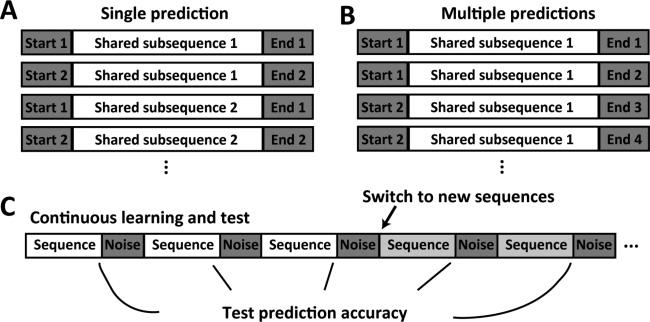
\includegraphics[width=0.8\columnwidth,clip=true]{figures/vlsi/sequences.jpg}}
%	\caption{Ακολουθίες συμβόλων για την προσομοίωση} \label{fig:sequences}
%\end{figure}
%
%Οι ακολουθίες φτιάχτηκαν έτσι ώστε να χρειάζεται ένα βάθος μνήμης τουλάχιστον 2 παρελθοντικών συμβόλων για την επιτυχή πρόβλεψη.
%Το πρώτο set ακολουθιών έχει δημιουργηθεί για να ελεγχθεί η δυνατότητα απλής πρόβλεψης, καθώς κάθε ακολουθία προσδιορίζεται πλήρως από τα πεδία ``Start'' και ``Shared Subsequence''.
%Αντιθέτως, στο δεύτερο set δύο ακολουθίες μπορεί να έχουν ίδια τα παραπάνω πεδία.
%Σε αυτή την περίπτωση το νευρωνικό δίκτυο θα πρέπει να επιτύχει την ορθή πρόβλεψη όλων των πιθανών καταλήξεων, δηλαδή την ταυτόχρονη πολλαπλή πρόβλεψη.
%Τέλος, ανάμεσα στις ακολουθίες προστέθηκε ένα σύμβολο θορύβου, ώστε να εξεταστεί η ανθεκτικότητα του συστήματος σε αυτόν.
%\begin{figure}[H]
%	\centering%
%	{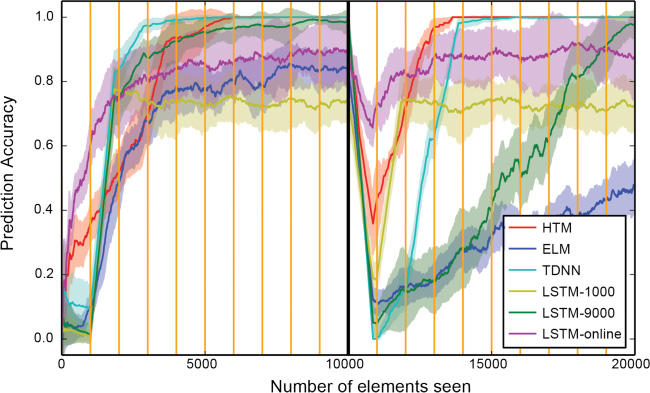
\includegraphics[width=0.7\columnwidth,clip=true]{figures/vlsi/single_prediction.jpg}}
%	\caption{Απόδοση διαφορετικών υλοποιήσεων για απλή πρόβλεψη} \label{fig:single-prediction}
%\end{figure}
%
%Στο σχήμα \eqref{fig:single-prediction} δίνεται η συγκριτική απόδοση των διαφορετικών υλοποιήσεων νευρωνικών δικτύων για το πρώτο set ακολουθιών.
%Τα δίκτυα που υλοποιούνται είναι το HTM, το ELM, το TDNN και το LSTM.
%Ο προσδιορισμός στο LSTM αφορά το πλήθος των δειγμάτων που χρησιμοποιούνται για retraining σε κάθε κατακόρυφη κίτρινη γραμμή του διαγράμματος.
%Στο στοιχείο 10000 που σημειώνεται με κάθετη κατακόρυφη γραμμή, αλλάζουν αμοιβαία τα δύο τελευταία σύμβολα κάθε ακολουθίας και μελετάται η προσαρμογή του δικτύου στο νέο input space.
%Βλέπουμε ότι το HTM πετυχαίνει αρχικά σε έναν ικανοποιητικό αριθμό δειγμάτων ακρίβεια $100\%$.
%Το πιο σημαντικό είναι, βέβαια, ότι μέσω online training αναπροσαρμόζεται ταχύτερα από κάθε άλλη υλοποίηση στο νέο χώρο ακολουθιών εισόδου.\\
%\begin{figure}[H]
%	\centering%
%	{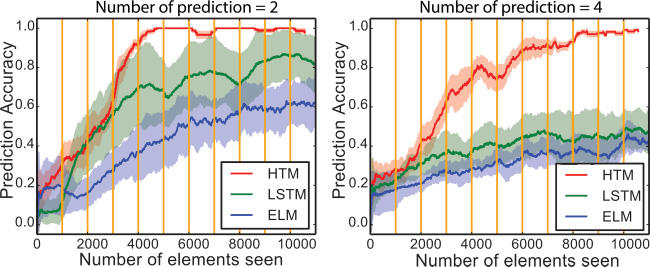
\includegraphics[width=0.8\columnwidth,clip=true]{figures/vlsi/multiple_predictions.jpg}}
%	\caption{Απόδοση δικτύων για πολλαπλές προβλέψεις} \label{fig:multiple-prediction}
%\end{figure}
%
%Οι πολλαπλές προβλέψεις εξετάζονται από το δεύτερο σετ και τα συγκριτικά αποτελέσματα για διπλή και τετραπλή πρόβλεψη δίνεται στο σχήμα \eqref{fig:multiple-prediction}.
%Όπως φαίνεται, το HTM είναι το μοναδικό σύστημα που πετυχαίνει μετά από κάποιο διάστημα ακρίβεια σχεδόν $100\%$.
%Αυτό απορρέει από την αναπαράσταση μέσω SDR και τη δυνατότητα του Temporal Pooler για πολλαπλές προβλέψεις.\\
%Στη συνέχεια, μελετήθηκε η απόδοση του HTM για ακολουθίες διαφορετικού μήκους.
%Ένα από τα τα σημαντικότερα στοιχεία του Temporal Pooler είναι η δυνατότητα αναπροσαρμογής online του «βάθους» μνήμης που χρησιμοποιείται για την πρόβλεψη.
%Έτσι, όπως παρατηρούμε και στο διάγραμμα \eqref{fig:sequence-order}, πετυχαίνει πρόβλεψη ακόμα και τάξης 100, που σημαίνει ότι απαιτείται μνήμη 99 συμβόλων για να προβλεφθεί επιτυχώς το τελευταίο.
%Το πλήθος των ακολουθιών που απαιτείται για να εκπαιδευτεί το σύστημα και να πετύχει ακρίβεια κοντά στο $100\%$ αυξάνει γραμμικά με την τάξη της ακολουθίας.
%\begin{figure}[H]
%	\centering%
%	{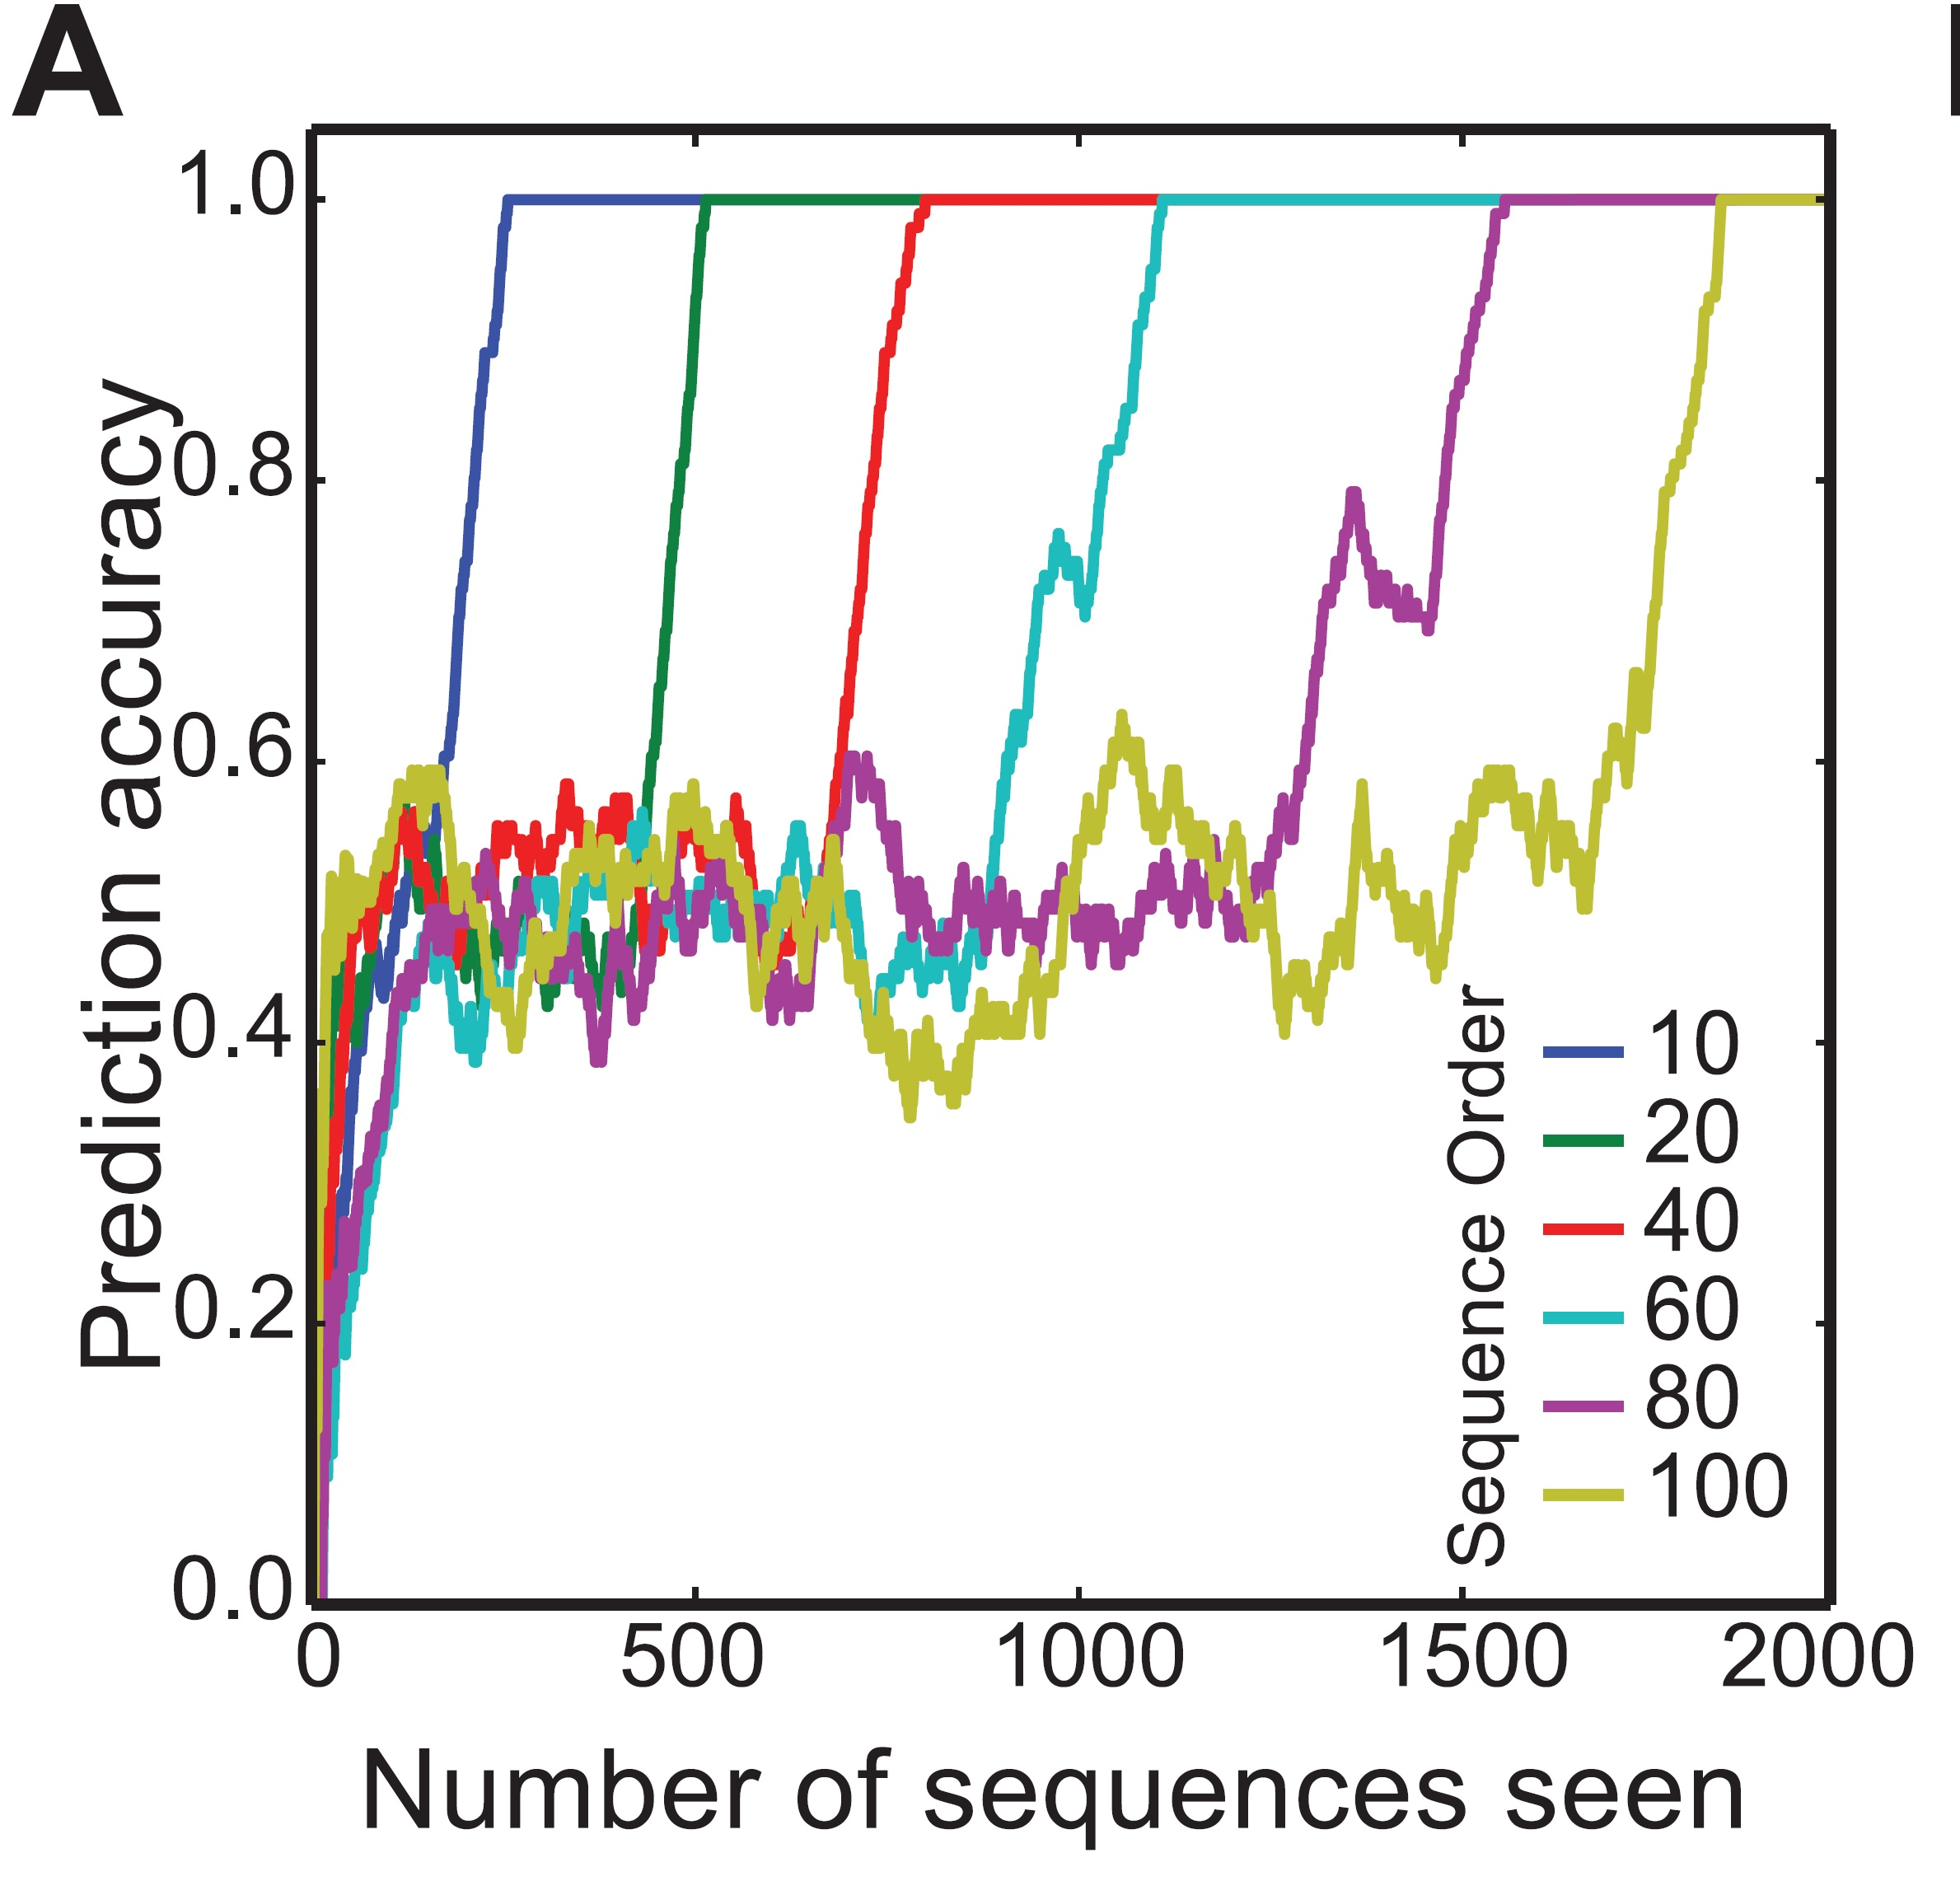
\includegraphics[width=0.4\columnwidth,clip=true]{figures/vlsi/sequence_order.jpg}}
%	\caption{Απόδοση HTM συναρτήσει της τάξης της ακολουθίας} \label{fig:sequence-order}
%\end{figure}
%
%Τέλος, τα διαφορετικά συστήματα εξετάστηκαν και ως προς την ανθεκτικότητα σε καταστροφή του δικτύου μέσω νεκρών νευρώνων.
%Το HTM έμεινε ανεπηρέαστο ακόμα για $30\%$ νεκρούς νευρώνες, συνθήκες κατά τις οποίες το ELM και το LSTM είχαν υποβαθμιστεί αρκετά.
%
%\begin{figure}[H]
%	\centering%
%	{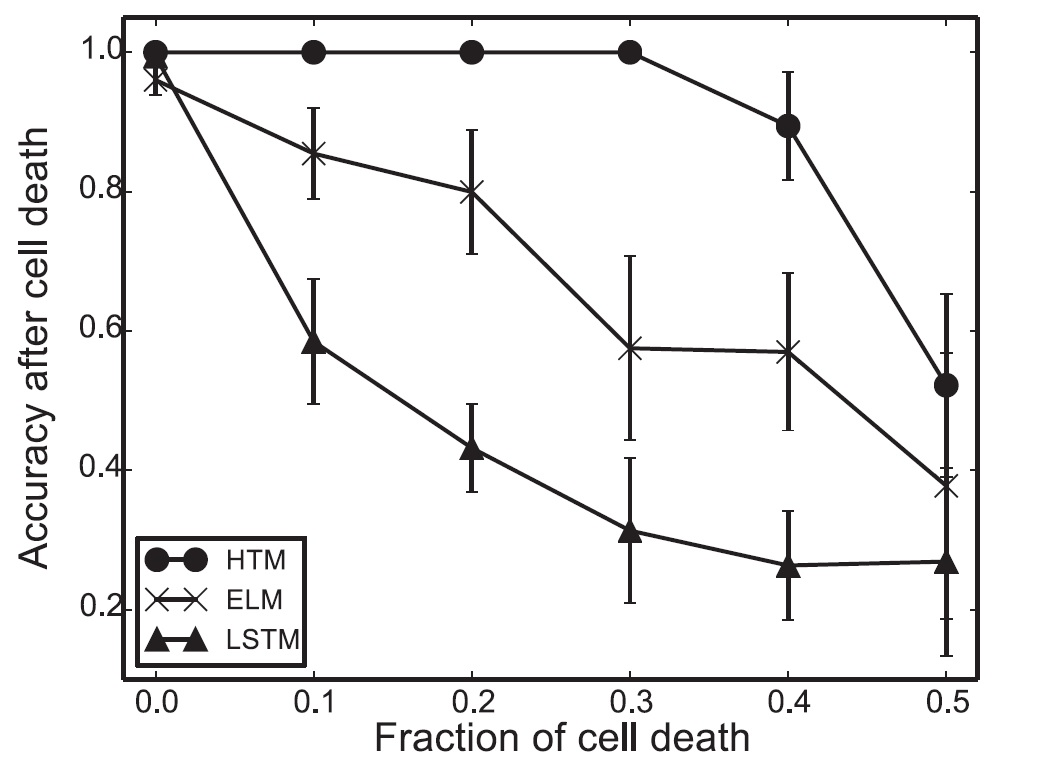
\includegraphics[width=0.4\columnwidth,clip=true]{figures/vlsi/cell_death.jpg}}
%	\caption{Ανθεκτικότητα υλοποιήσεων σε νεκρούς νευρώνες} \label{fig:cell-death}
%\end{figure}
%
%
%\subsubsection{Πρόβλεψη της ζήτησης taxi στη Νέα Υόρκη}
%
%Το Hierarchical Temporal Memory δοκιμάστηκε και σε πραγματικά streaming δεδομένα.
%Πιο συγκεκριμένα, ζητήθηκε η πρόβλεψη της ζήτησης στα taxi της Νέας Υόρκης 2.5 ώρες πριν την πραγματική μέτρηση.
%Η ζήτηση ποσοτικοποιήθηκε ως η συνολική εξυπηρέτηση πελατών σε ένα χρονικό παράθυρο 30 λεπτών.
%Εξετάστηκαν διάφοροι τύποι νευρωνικών δικτύων, καθώς και το στατιστικό μοντέλο ARIMA.
%%Όπως παρατηρούμε από την εικόνα \ref{fig:taxi_accuracy}, το HTM πέτυχε το μικρότερο απόλυτο σφάλμα πρόβλεψης (της τάξης του $0.08\%$ ).\\
%
%\begin{figure} [H]
%	\centering%
%	\begin{subfigure}{0.5\columnwidth}
%		{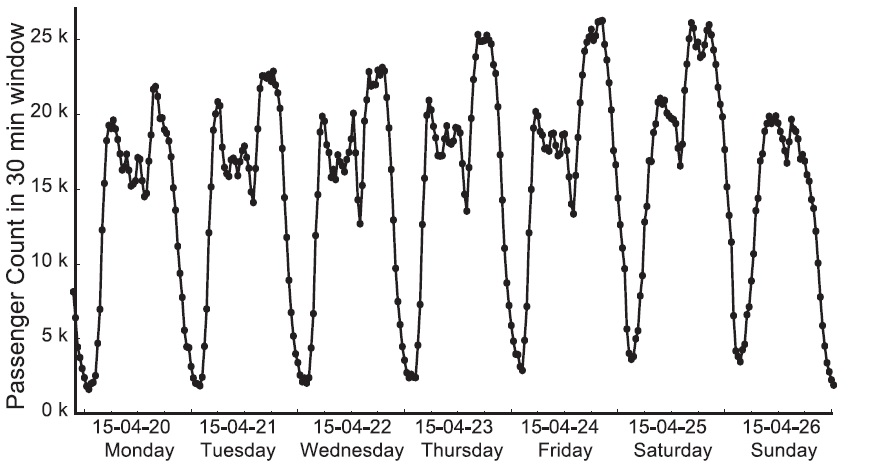
\includegraphics[width=\columnwidth,clip=true]{figures/vlsi/taxi_demand.jpg}}
%		\caption{Διάγραμμα ζήτησης}
%		\label{fig:taxi_demand}
%	\end{subfigure}%
%	\begin{subfigure}{0.5\columnwidth}
%		\centering
%		{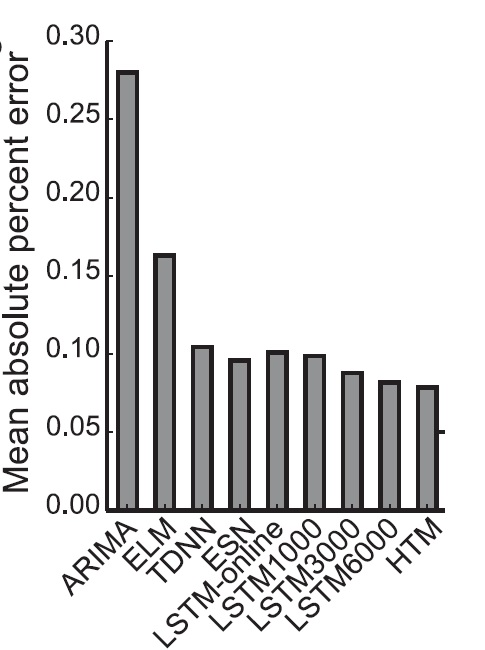
\includegraphics[width=0.5\columnwidth,clip=true]{figures/vlsi/taxi_accuracy.jpg}}
%		\caption{Μέσο απόλυτο σφάλμα}
%		\label{fig:taxi_accuracy}
%	\end{subfigure}
%	\caption{Πρόβλεψη ζήτησης των taxi}
%	\label{fig:taxi_simulation}
%\end{figure}
%
%Στη συνέχεια, τα δεδομένα εισόδου τροποποιήθηκαν τεχνητά ανεβάζοντας ή μειώνοντας τη ζήτηση κατά $20\%$ σε διαφορετικές χρονικές περιόδους εντός κάθε μέρας.
%Στόχος ήταν να μελετηθεί η προσαρμογή του δικτύου στις νέες (τεχνητές) συνήθειες των επιβατών taxi της Νέας Υόρκης.
%Η αλλαγή πραγματοποιήθηκε την 1η Απριλίου και εντός 2 βδομάδων το σύστημα HTM αναπροσάρμοσε το μοντέλο του, ώστε να πετυχαίνει εκ νέου σωστές προβλέψεις.
%Σε αντίθεση, το LSTM είτε απέτυχε να επανέρθει, είτε χρειάστηκε πολύ περισσότερο διάστημα για retraining των παραμέτρων του.
%
%\begin{figure}[h]
%	\centering%
%	{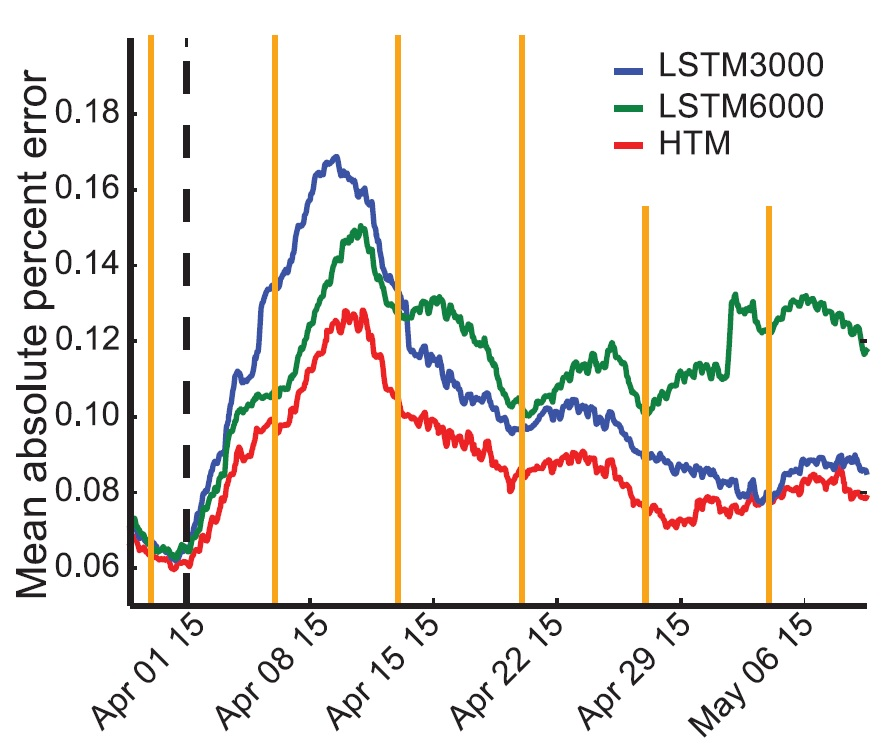
\includegraphics[width=0.4\columnwidth,clip=true]{figures/vlsi/taxi_adaptation.jpg}}
%	\caption{Προσαρμογή δικτύων σε μεταβολή της ζήτησης}
%	\label{fig:taxi-adaptation}
%\end{figure}
